\chapter{Expressive words and sentence final particles} \label{chap:ideophones.sfp}
This chapter comprises four sections: §\ref{sec:idph} discusses ideophones, §\ref{sec:other.expressive} presents expressive words lacking specific ideophonic properties (interjections and calling sounds), §\ref{sec:fillers} and §\ref{sec:sfp} describe sentence final particles and their contribution to the expression of modality and evidentiality.

\section{Ideophones} \label{sec:idph} 
Ideophones in Japhug constitute a particularly large part of speech, and can be unambiguously defined on the basis of morphological criteria. The present section builds on previous research \citep{jackson04zhuangmaoci, japhug14ideophones}), but is based on a  larger corpus of ideophones.

\subsection{Ideophonic stem morphology} \label{sec:ideo:morpho}
Cross-linguistic definitions have been proposed for ideophones; for instance, according to \citet[2]{dingemanse14}, they are `marked words that depict sensory imagery'.  While  Japhug ideophones do indeed fit this description, in this grammar a language-particular definition is adopted. 

Ideophones often have specific morphology, which differs from the rest of the lexicon (\citealt{diffloth76expressives} and  \citealt{zwicky87expressive}). This is the case in Gyalrong languages (\citealt[3--4]{jackson04zhuangmaoci}), and ideophones are thus defined in this grammar (following \citealt{japhug14ideophones}) as words derived from monosyllabic ideophonic roots that can undergo the morphological alternations described in this section. 

\tabref{tab:ideo.morpho1} presents the ten ideophonic patterns attested in Japhug. Since these patterns involve several types of partial reduplication, a set of symbols are used to represent the elements of the root that are targeted by reduplication: $C_i$ represents initial clusters (or single consonants), $C_f$ codas, $V$ the main vowel and $R$ the complete ideophonic root.

\begin{table}
\caption{Ideophonic morphology in Japhug} \label{tab:ideo.morpho1}
\begin{tabular}{llllll}
\lsptoprule
&pattern & example& meaning  \\
\midrule
I& $R$ & \forme{zjaŋ} &semelfactive \\
II&$R.R$ & \forme{zjaŋ.zjaŋ} &stative \\
III&$R$.\forme{nɤ}.$R$ & \forme{zjaŋ.nɤ.zjaŋ} & action with rhythm \\
&&&and/or motion \\
IV&$R$.\forme{nɤ.l}$VC_f$ & \forme{zjaŋ.nɤ.laŋ}&   action in disorderly fashion \\
V&\forme{pʰɯ}.$R$ & \forme{pʰɯ.zjaŋ} & semelfactive, intensive \\
VI&\forme{mɤlɤ}.$R$ & \forme{mɤlɤ.zjaŋ} & stative, intensive \\
VII&$R$\forme{ɯ}.$C_f$ \forme{i} & \forme{zjaŋɯ.ŋi} &progressive change of state  \\
VIII&$C_i$\forme{ɯ}$C_f$\forme{ɯ}.$C_i$\forme{a}$C_f$\forme{i} &  \forme{zjɯŋɯ.zjaŋi} & stative, in quantity, in disorder\\
&$R$\forme{ɯ}.$C_i$\forme{a}$C_f$\forme{i}&\\
IX&$R$\forme{i}.\forme{nɤ}.$R$\forme{i} & \forme{zjaŋi.nɤ.zjaŋi} & action with fast motion \\
X&$RRR(*)$&&onomatopoeia \\
\lspbottomrule
\end{tabular}
\end{table}

This system is not specific to Japhug: patterns I, II, III, IV and VII have direct correspondences in Tshobdun \citep[3--4]{jackson04zhuangmaoci}. Patterns V and VI express an intensive meaning in comparison with the corresponding semelfactive (pattern I) and stative (pattern II). No equivalent pattern exists in Tshobdun. The \forme{-nɤ-} element in patterns III, IV and IX is related to the additive \forme{nɤ} (§\ref{sec:additive.nA}).

All patterns (except X) are illustrated with an example using the root \idroot{zjaŋ}  `tall'. Example sentences for each of these forms and more detailed accounts of their semantics are provided in §\ref{sec:ideo.regular}.
   
 
\subsection{Regular derivations} \label{sec:ideo.regular}
 Although most ideophonic patterns are attested in the text corpus, it is difficult to find real examples of all regular derivations from one particular root. For ease of presentation, we cite example sentences with complex ideophones based on a single root, \idroot{zjaŋ}  `tall',\footnote{This root is not used to illustrate pattern X (§\ref{sec:ideo.X}), which is semantically restricted. } and thus most of these examples are elicited.\footnote{They are however not translated: I asked my main consultant Tshendzin to produce sentences illustrating each of the possible patterns of the root \idroot{zjaŋ}. } Ideophones are glossed by \textsc{idph}, followed by the number of the pattern, and a brief translation of the general meaning of the ideophonic root.

The basic meaning of the ideophonic root \idroot{zjaŋ}  `tall' was glossed by Tshendzin as (\ref{ex:zjaN.expl}).

\begin{exe} 
\ex \label{ex:zjaN.expl}
\gll ɯ-zda ra sɤz kɯ-mbro kɯ-fse \\
\textsc{3sg}.\textsc{poss}-companion \textsc{pl} \textsc{comp} \textsc{sbj}:\textsc{pcp}-be.tall \textsc{sbj}:\textsc{pcp}-be.like \\
\glt `Taller or higher than the others.' (elicited) 
\end{exe}

There is a series of ideophonic roots that are related to \idroot{zjaŋ} by other type of processes (\tabref{tab:zjaN.tsjaN}, §\ref{sec:idph.gradation}).

 \subsubsection{Pattern I} \label{sec:ideo.I}
Pattern I, which consists of the bare ideophonic root, is combined with predicates in the Aorist or Inferential to express an action occurring suddenly, as in (\ref{ex:ideo1}). The form \forme{zjaŋ} means that the action of the sentence resulted in the main referent becoming taller than its surrounding.

\begin{exe} 
\ex \label{ex:ideo1}
\gll \textbf{zjaŋ} ʑo tɤ-ndzur  \\
\textsc{idph}(I):tall \textsc{emph} \textsc{aor}-stand \\
\glt `He stood up suddenly, and [appeared to be] very tall.'  (elicited)
\end{exe}
 
\subsubsection{Pattern II} \label{sec:ideo.II}
Pattern II with plain reduplication indicates a state. It is by far the most common ideophonic pattern in texts and it is attested for most ideophonic roots.  It generally describes  a permanent state (as in \ref{ex:RJWRJri} below).

When an ideophone in pattern II is used with a lexical verb, it can describe a state resulting from the action indicated by the main verb (\japhug{rmbɯ}{heap up} in \ref{ex:zjaNzjaN3}).

  \begin{exe} 
\ex  \label{ex:zjaNzjaN3}
\gll  tɕe zjaŋzjaŋ ʑo kɯ-pa to-rmbɯ-nɯ \\
\textsc{lnk} \textsc{idph}(II):tall \textsc{emph} \textsc{inf}:\textsc{stat}-\textsc{aux} \textsc{ifr}-pile.up-\textsc{pl} \\
 \glt `[The villagers] had piled [the hay] up very high.' (150902 liaozhai lang-zh)'
\japhdoi{0006340\#S24}
  \end{exe}
  
A handful of deideophonic verbs in \forme{a-} and \forme{nɤ-} can be built from pattern II ideophones (§\ref{sec:a.nA.deidph}).
 
 The reduplicated form in pattern II is in most cases a complete reduplication. Not only the onset, but also the vowel as well as the final consonant are copied, even in the case of initial clusters, as in \idroot{zɟraŋ} $\rightarrow$ \forme{zɟraŋzɟraŋ} `bulging, swollen'. 

Nevertheless, we do observe some phonetic attrition in the case of  the codas \forme{-t}, \forme{-ɣ} and \forme{-β}. Final \forme{-t} is generally deleted regardless of the following consonant, as in  \idroot{xʂɤt} $\rightarrow$ \forme{xʂɤxʂɤt} `long, thin and flexible'. An exception, which involves an ideophone without initial cluster, is \forme{cotcot} `small and cute'.

Final \forme{-β} generally disappears in the reduplicated syllable when the onset of the ideophonic root contains a labial (§\ref{sec:heterosyllabic.clusters}), as in \idroot{bɤβ} $\rightarrow$  \forme{bɤbɤβ} `stubborn, bulky'. This rule is however only optional, and \forme{bɤβbɤβ} is also attested.

Final \forme{-ɣ} is generally deleted when the onset contains a velar (§\ref{sec:heterosyllabic.clusters}) as in \idroot{gɤɣ} $\rightarrow$ \forme{gɤgɤɣ} `moving with difficulty, unstable on its feet'. This rule is also optional.

Another type of phonetic reduction optionally appears with a few ideophones with open rhymes in \forme{-i} and a initial cluster with medial \forme{-l-} or \forme{-r-}. The medial is deleted and the rhyme is replaced by \forme{-ɯ}, following the regular process of partial reduplication common in verbal morphology (§\ref{sec:partial.redp}). Examples of this phenomenon include for instance \idroot{ʁɟri} $\rightarrow$ \forme{ʁɟɯʁɟri} `fat, soft and wet' and  \idroot{qli} $\rightarrow$ \forme{qɯqli} `staring without moving'.

  \begin{exe} 
\ex  \label{ex:RJWRJri}
\gll ɯ-βri nɯra kú-wɣ-rtoʁ qʰe ɲɯ-ɤcilaj ʑo qʰe, nɤkinɯ, ʁɟɯʁɟri ʑo ɲɯ-pa. \\
\textsc{3sg}.\textsc{poss}-body \textsc{dem}:\textsc{pl} \textsc{ipfv}-\textsc{inv}-look \textsc{lnk} \textsc{sens}-be.wet \textsc{emph} \textsc{lnk} \textsc{filler} \textsc{idhp}:II:fat.soft.wet \textsc{emph} \textsc{sens}-\textsc{aux} \\
\glt `The body [of the gecko] looks wet, it is wet and soft.' (28-tshAwAre) 	\japhdoi{0003722\#S37}
  \end{exe}

\subsubsection{Pattern III} \label{sec:ideo.III}
Pattern III is formed by reduplicating the ideophonic root with the additive marker \forme{nɤ} (§\ref{sec:additive.nA}) inserted in between. It depicts a rhythmic action or a constant motion as in (\ref{ex:ideo3}), depending on the semantics of the root.   
  
 \begin{exe} 
\ex  \label{ex:ideo3}
\gll  mbro ɯ-taʁ to-ɕe tɕe \textbf{zjaŋnɤzjaŋ} jɤ-ari-ndʑi   \\
horse \textsc{3sg}-on  \textsc{ifr}:\textsc{up}-go \textsc{lnk} \textsc{idph}(III):tall  \textsc{aor}-go[II]-\textsc{du} \\
\glt `He mounted the horse, and  they went there, very tall.'  (elicited)
 \end{exe} 
 
 Deideophonic verbs in \forme{ɣɤ-} and \forme{sɤ-} (§\ref{sec:GA.sA.deidph}) and \forme{nɯ-} (§\ref{sec:nW.deidph}) are built from pattern III ideophones, without additive \forme{nɤ}.
 
  Pattern III also allows a variant $RR$-\forme{nɤ}-$RR$ with double reduplication of the ideophonic root, with an intensive meaning. For instance \forme{pɣɤlnɤpɣɤl} `(walking) with big strides' has the slightly different meaning `(running) with big strides' with double reduplication (\ref{ex:pGAlnApGAl}).
  
\begin{exe} 
\ex \label{ex:pGAlnApGAl}
\gll `wo a-mu ma-pɯ-tɯ-ʑɣɤ-sat tɕe aʑo pjɯ-nɯ-ɣi-a ŋu' to-ti. pɣɤlpɣɤlnɤpɣɤlpɣɤl pjɤ-nɯ-ɣi. \\
\textsc{interj} \textsc{1sg}.\textsc{poss}-mother \textsc{neg}-\textsc{imp}-2-\textsc{refl}-kill \textsc{lnk} \textsc{1sg} \textsc{ipfv}:\textsc{down}-\textsc{vert}-come-\textsc{1sg} be:\textsc{fact} \textsc{ifr}-say \textsc{idph}(III):with.big.strides \textsc{ifr}:\textsc{down}-\textsc{auto}-come \\
\glt `She said ``Mother, don't commit suicide, I am coming back'' and came back running in big strides.' (2003 kAndZWsqhaj2)
\end{exe} 
 
 
   \subsubsection{Pattern IV} \label{sec:ideo.IV}
Pattern IV is formed by combining with the ideophonic root, the additive \forme{nɤ} (§\ref{sec:additive.nA}) and a partial copy of the ideophonic root replacing the onset by \forme{l\trt}, a pattern reminiscent of some distributed action verbs (§\ref{sec.distributed.action.l}). It describes an action involving motion  occurring in disorderly fashion with intermittent changes of state. In (\ref{ex:ideo4}) the form  \forme{zjaŋnɤlaŋ} can be used to depict a drunk person who stumbles from time to time while walking, so that he seems taller at one time and shorter at another time.
 
  \begin{exe} 
\ex  \label{ex:ideo4}
\gll  zjaŋnɤlaŋ ɲɯ-ŋke   \\
     \textsc{idph}(IV):tall \textsc{sens}-go  \\
\glt `He is walking unsteadily, very tall.'   (elicited)
 \end{exe} 
 
Deideophonic verbs in \forme{ɣɤ-} and \forme{sɤ-} can be build from pattern IV ideophones (§\ref{sec:GA.sA.deidph}), without insertion of the additive.

\subsubsection{Pattern V} \label{sec:ideo.V}
 Pattern V, made of the ideophonic root prefixed with the element \forme{pʰɯ\trt}, is similar to pattern I (§\ref{sec:ideo.I}) semantically, but it is more rarely used; it indicates a more sudden action and/or one carried out to a higher degree.
 
  \begin{exe} 
\ex  \label{ex:ideo5}
\gll  pʰɯzjaŋ ʑo tɤ-ndzur   \\
\textsc{idph}(V):tall \textsc{emph} \textsc{aor}-stand \\
\glt `He stood up suddenly, and [appeared to be] very tall.'  (elicited)
\end{exe}
 
This pattern occurs in particular with onomatopoeic ideophones, such as \idroot{qʰloŋ} `splashing' (\ref{ex:phWqhloN}).

  \begin{exe} 
\ex  \label{ex:phWqhloN}
\gll nɯ pʰɯqʰloŋ ʑo pjɤ-ɣɤrɤt \\
\textsc{dem} \textsc{idph}(V):splashing \textsc{emph} \textsc{ifr}-throw \\
\glt `He threw [the bag into the water], making a sudden splashing noise.' (150824 kelaosi-zh) \japhdoi{0006276\#S146}
 \end{exe}
 
 The most common pattern V ideophone is \forme{pʰɯɕlaʁ}  from \idroot{ɕlaʁ} `suddenly', which has  the \forme{ɣɤ-} and \forme{sɤ-}  denominal forms (§\ref{sec:GA.sA.deidph}) \forme{ɣɤpʰɯɕlaʁ} `moving/working quickly, hardworking' and \forme{sɤpʰɯɕlaʁ} `do $X$ quickly (not lingering)'.

\subsubsection{Pattern VI} \label{sec:ideo.VI}
Pattern VI, with the root prefixed by \forme{mɤlɤ\trt}, describes a state like pattern II, but differs from it in that it expresses a higher degree. In addition, it can be used to express the result of a change of state with the verb \japhug{aβzu}{become, grow} as in (\ref{ex:ideo6}). It is the rarest of all ideophonic patterns, not attested in the Japhug text corpus.

 \begin{exe} 
\ex  \label{ex:ideo6}
\gll a-ɣe \textbf{mɤlɤzjaŋ} ʑo tʰɯ-aβzu   \\
\textsc{1sg}.\textsc{poss}-grandson \textsc{idph}(VI):tall \textsc{emph} \textsc{aor}-become \\
\glt `My grandson has become very tall.'  (elicited)
 \end{exe}

  \subsubsection{Pattern VII} \label{sec:ideo.VII}
In pattern VII, the coda of the root ($C_f$; if no coda is present, a \ipa{w} is inserted, §\ref{sec:ideo.VIII}) is resyllabified as onset of a syllable with the vowel \forme{ɯ}, and then reduplicated with the vowel \forme{i} following the pattern $C_fV$.$C_f$\forme{ɯ}.$C_f$\forme{i}. It  expresses a progressive change of state, involving in some case slow motion as in (\ref{ex:ideo7}).
 
  \begin{exe} 
\ex  \label{ex:ideo7}
\gll  zjaŋɯŋi ʑo jɤ-ari   \\
\textsc{idph}(VII):tall  \textsc{emph} \textsc{aor}-go[II] \\
\glt `He went away slowly, looking taller than rest.'  (elicited)
 \end{exe}
 
  \subsubsection{Pattern VIII} \label{sec:ideo.VIII}
 Pattern VIII  depicts a state involving a lot of referents having the property described by the ideophone, but spread out spatially in a disorderly fashion. 

The formula $R$\forme{ɯ}.$C_i$\forme{a}$C_f$\forme{i} in \tabref{tab:ideo.morpho1} applies to ideophonic roots  which do  not have \ipa{a} as their main vowel, for instance \idroot{zjɤɣ} (whose meaning is almost identical to that of \idroot{zjaŋ}) has the form \forme{zjɤɣ.ɯ.zjaɣ.i}. When the main vowel is \ipa{a}, the formula is $C_i$\forme{ɯ}$C_f$\forme{ɯ}.$C_i$\forme{a}$C_f$\forme{i}. Thus, the pattern VIII of  \idroot{zjaŋ} is \forme{zjɯ.ŋɯ.zja.ŋi}. This form means that in a group of unique entities, some are tall and some are short, but  they are unevenly spread (\ref{ex:ideo8}).
	
\begin{exe} 
\ex  \label{ex:ideo8}
\gll  zjɯŋɯzjaŋi ɲɯ-xcat \\
\textsc{idph}(VIII):tall \textsc{sens}-be.many \\
\glt `There are many [people], some taller and some shorter.'   (elicited)
  \end{exe}
	 
 Tshendzin glossed the meaning of (\ref{ex:ideo8}) as follows (\ref{ex:zjWNWzjaNi:expl}).
 
 \begin{exe} 
\ex  \label{ex:zjWNWzjaNi:expl}
\gll  tsuku kɯ-mbro tsuku kɯ-mbɤr kɯ-fse   \\
 some \textsc{sbj}:\textsc{pcp}-be.tall some \textsc{sbj}:\textsc{pcp}-be.short \textsc{sbj}:\textsc{pcp}-be.like \\
 \glt `Some tall and some short.'    (elicited)
  \end{exe}  

  In cases where the ideophonic root has no coda, the consonant \ipa{w} replaces $C_f$ in patterns VII and VIII. For instance, /\forme{ʂχi}/ `with big holes, with big nostrils' has the pattern VIII form \forme{ʂχɯwɯʂχawi} `full of holes everywhere' (\ref{ex:sxXwwWsxWawi}).

\begin{exe} 
\ex \label{ex:sxXwwWsxWawi}
\gll nɯnɯ ɯ-ŋgɯ ri ɕ-tu-ndze tɕe ku-rɤʑi ɲɯ-ɕti tɕe, (...) nɯnɯtɕu aʁɤndɯndɤt ʂχɯwɯʂχawi ɲɯ-sɯ-spoʁ tɕe \\
\textsc{dem} \textsc{3sg}.\textsc{poss}-in \textsc{loc} \textsc{tral}-\textsc{ipfv}-eat[III] \textsc{lnk} \textsc{ipfv}-stay \textsc{sens}-be.\textsc{aff}:\textsc{fact} \textsc{lnk} {  } \textsc{dem}:\textsc{loc} everywhere \textsc{idph}(VIII):with.holes \textsc{ipfv}-\textsc{caus}-have.a.hole \textsc{lnk} \\
\glt `[The species of ants called \forme{cɤmi qro}] goes into wood and eats it, and stays in there, (...) and makes holes everywhere in it.' (26-qro)
\japhdoi{0003682\#S89}
\end{exe} 

\subsubsection{Pattern IX} \label{sec:ideo.IX}
Pattern IX is formally similar to pattern III except that \ipa{i} is added after each reduplicant of the ideophonic root. Semantically, it indicates that the entity presenting the property described by the ideophonic root undergoes a fast motion.

\begin{exe} 
\ex  \label{ex:ideo9}
\gll  mbro ta-nɯmbrɤpɯ tɕe zjaŋinɤzjaŋi ʑo jɤ-ɕqʰlɤt   \\
horse \textsc{aor}:3\flobv{}-ride \textsc{lnk} \textsc{idph}(IX):tall \textsc{emph} \textsc{aor}-disappear \\
\glt `He mounted the horse and disappeared quickly (in the horizon), very tall.'  (elicited)
 \end{exe}

 
\subsubsection{Pattern X} \label{sec:ideo.X}
Pattern X involves reduplication of the ideophonic root three or more times (it was not considered to be an ideophonic pattern in \citealt{japhug14ideophones}). It is the only domain of Japhug grammar where triplication is allowed,\footnote{Another language in which ideophone triplication has been documented is Chintang \citep{rai06triplication}.
} unlike the Mazur variety of Stau, where triplication occurs in finite verb forms \citep{gates17triplication}.

Pattern X differs from all preceding patterns in that it is semantically restricted to onomatopoeia (\ref{ex:cutcutcut}) and endopathic ideophones (ie. ideophones expressing inner sensations such as cold or pain) (\ref{ex:zWrzWrzWr}), and nearly always select \japhug{ti}{say} as light verb (§\ref{sec:idph.ti}). Lexical verbs are also attested with pattern X ideophones (\ref{ex:rCWB4.pjWlAt}), though more rarely.
 
\begin{exe}
\ex \label{ex:cutcutcut}
\gll    tu-mbri nɯra cutcutcut ʑo tu-ti ɲɯ-ŋu  \\
  \textsc{ipfv}-call \textsc{dem}:\textsc{pl} \textsc{idph}(X):cry \textsc{emph} \textsc{ipfv}-say \textsc{sens}-be \\
\glt  `When it calls it makes `\forme{cut cut cut}'.' (24-ZmbrWpGa) 	\japhdoi{0003628\#S8}
\end{exe}

\begin{exe}
\ex \label{ex:zWrzWrzWr}
\gll ɲɯ-kɯ-sɤŋo tɕe, nɯ nɯ-ɬoʁ tɕe, zɯrzɯrzɯr tu-ti qʰe tɕendɤre tɤ-ndɤr ɲɯ-ɬoʁ ɕti.	\\
\textsc{ipfv}-\textsc{genr}:S/O-listen \textsc{lnk} \textsc{dem} \textsc{aor}-come.out \textsc{lnk} \textsc{idph}(X):itchy.feeling \textsc{ipfv}-say \textsc{lnk}  \textsc{lnk} pimple \textsc{ipfv}-come.out be:\textsc{aff}:\textsc{fact} \\
\glt `When it appears, one has an itchy feeling, and a pimple appears.' (25-khArWm) 	\japhdoi{0003644\#S4}
\end{exe}

The triplication (reduplication at will) of the root expresses either repeated action like pattern III, or a continuous and unceasing state. Some pattern X ideophones are reduplicated four (\ref{ex:rCWB4.pjWlAt}) or more (\ref{ex:ZeZeZeZe}) times. 

\begin{exe}
\ex \label{ex:rCWB4.pjWlAt}
\gll tɤɕi qaj nɯ tɤtɤɣ ɯ-ŋgɯ rɕɯβrɕɯβrɕɯβrɕɯβ ʑo pjɯ-lɤt nɯ, ɯ-zgra nɯ pjɤ-sɤ-mtsʰɤm.  \\
barley wheat \textsc{dem} cupboard \textsc{3sg}.\textsc{poss}-in \textsc{idph}(X):rustling \textsc{emph} \textsc{ipfv}-release \textsc{dem} \textsc{3sg}.\textsc{poss}-noise \textsc{dem} \textsc{ifr}.\textsc{ipfv}-pro-hear \\
\glt `(In the night), one could hear the rustling noise of the [one-legged demon]$_i$ pouring barley and wheat grains into the cupboard (of the woman with whom he$_i$ was having a relationship). (140510 rkoNJAl) \japhdoi{0003943\#S30}
\end{exe}

Not all onomatopoeia are realistic descriptions of natural sounds. In (\ref{ex:ZeZeZeZe}) we find an ideophonic root \idroot{ʑe}* describing the supposed minute sound made by the quick motion of the legs of a millipede.

\begin{exe}
\ex \label{ex:ZeZeZeZe}
\gll kú-wɣ-rtoʁ tɯ-mɲaʁ kɯ ɯ-mɤlɤjaʁ ra mɯ́j-saχsɤl ʑo ri, ``ʑeʑeʑeʑeʑeʑe" ʑo tu-ti ju-ɕe qʰe, ɯ-tɯ-mbjom sɤre ʑo \\
\textsc{ipfv}-\textsc{inv}-look \textsc{genr}.\textsc{poss}-eye \textsc{erg} \textsc{3sg}.\textsc{poss}-limb \textsc{pl} \textsc{neg}:\textsc{sens}-be.clear \textsc{emph} \textsc{lnk} \textsc{idph}(II):sound \textsc{emph} \textsc{ipfv}-say \textsc{ipfv}-go \textsc{lnk} \textsc{3sg}.\textsc{poss}-\textsc{nmlz}:\textsc{deg}-be.quick be.ridiculous:\textsc{fact} \textsc{emph} \\
\glt `(Of a type of small millipede) Looking at it, its feet are not clearly visible, but it moves making \forme{ʑeʑeʑeʑeʑeʑe}, extremely quickly.' (28-kWpAz)
\japhdoi{0003714\#S142}
\end{exe} 

Some of the roots used in pattern X are polysyllabic (see for instance \forme{dudut} in §\ref{sec:underived.expressive.nouns}), in which case the ideophone can only be reduplicated two times.

  
\subsection{Semantic categories}
Japhug ideophones are used for describing various features including sound, colour, shape, texture, attitude or mood, and some ideophones are multimodal, referring to combination of several types of sensory information.

\citet[663]{dingemanse12ideo} proposed the hierarchy (\ref{ex:ideo.hierarchy}) according to which, if a particular language possesses ideophones belonging to a particular class in this hierarchy, it will also present ideophones for all the lower classes. All categories are exemplified in Japhug.

\begin{exe} 
\ex  \label{ex:ideo.hierarchy}
\glt \textsc{sound} > \textsc{motion} > \textsc{visual patterns}  > \textsc{other sensory perceptions} > \textsc{inner feelings and cognitive states}
\end{exe}

Onomatopoeic ideophones include for instance \idroot{qʰloŋ} `splashing' (\ref{ex:phWqhloN}, §\ref{sec:ideo.V}) or \idroot{tɕʰɯŋ} `metal clinking'. 

In addition to sounds, ideophonic roots also describe shapes (for instance \forme{boŋboŋ} `ovoid'), specific hues of colour (\forme{smɯɣsmɯɣ} `fresh green'), touch (\forme{brɯɣbrɯɣ} `rough, covered in small pimples'), temperature (\forme{xɯβxɯβ} `warm'), size (\forme{scraʁscraʁ} `very small, close to the ground'), quantity (\forme{ʑɯβʑɯβ} `many (people, object) standing/in upright position'), attitudes (\forme{dɣɤrdɣɤr} `agape, in a daze, looking stupid', \forme{ɕquɕqu} `frowning'), pain (\forme{ɕɲɯɣ} `intense and sudden pain'), body position (\forme{ɕpʰɤβɕpʰɤβ} `lying on the ground, motionless') and also cognitive states (\forme{ɬɤɬɤt} `free from worry').


Ideophonic roots often combine several parameters. For instance, \forme{ɕɣaʁɕɣaʁ} `sharp and shiny (of fangs)' encodes both shape and hue.

%ɕphɤβɕphɤβ  形容卧在地上不动的样子
%ɕqlɤβɕqlɤβ 形容不高兴的眼神的样子

It appears that there are no ideophonic \textit{roots} specifically dedicated to expressing motion; however, dynamic ideophonic patterns (I, III, IV, IX) applied to ideophones describing sound or shapes often add a motional imagery. For instance, the root \idroot{xɯr} means `round' in pattern II, but `rotating, turning' in pattern III (\ref{ex:xWrnAxWr}, §\ref{sec:nW.deidph}) and IX (\ref{ex:xWrinAxWri}).

\begin{exe} 
\ex  \label{ex:xWrinAxWri}
\gll ɯ-mɤlɤjaʁ kɯra nɤ kɯra tu-ste qʰe tɕe, iɕqʰa staχpɯrɟɤskʰi ɣɯ ɯ-jwaʁ nɯ xɯrinɤxɯri ʑo tu-sɯ-mtɕɯr. \\
\textsc{3sg}.\textsc{poss}-limb \textsc{dem}.\textsc{prox}:\textsc{pl} \textsc{add}  \textsc{dem}.\textsc{prox}:\textsc{pl} \textsc{ipfv}-do.like[III] \textsc{lnk} \textsc{lnk} the.aforementioned plant.name \textsc{gen} \textsc{3sg}.\textsc{poss}-leave \textsc{dem} \textsc{idph}(IX):round \textsc{emph} \textsc{ipfv}-\textsc{caus}-turn \\
\glt `[There is a species of insect which] does this with its legs repeatedly, and rotates the leaves of the \forme{staχpɯrɟɤskʰi} very quickly.' (18-NGolo)
\japhdoi{0003530\#S128}
\end{exe} 

Some ideophones, however, can have an auditory interpretation competing with many other ones. Thus, \idroot{bɤβ} in pattern II form \forme{bɤbɤβ} can designate many objects clustered together (like mushrooms) (\ref{ex:kAmWsthWsthaB}, §\ref{sec:recip.amW.indirective} and \ref{ex:WtaR.ra.Wmat}, §\ref{sec:plural.determiners}), a stubborn person or a heavy and cumbersome object depending on the context. 

With a dynamic pattern such as I or III, it can be interpreted as designating the noise made by a heavy object falling from a high place as in (\ref{ex:bAB.Zo.paBde}), a meaning shared with the deideophonic verbs \forme{sɤbɤbɤβ} and \forme{nɯbɤβ} (see the examples in  \ref{ex:nWbAB.bABnAbAB}, §\ref{sec:nW.deidph}).

\begin{exe}
\ex \label{ex:bAB.Zo.paBde}
\gll mbro kɯ [...] tɕʰeme nɯ bɤβ ʑo pjɤ-βde qʰe \\
horse \textsc{erg} { } girl \textsc{dem} \textsc{idph}(I):heavy.object.falling \textsc{emph} \textsc{ifr}:\textsc{down}-throw \textsc{lnk}  \\
\glt `The horse (...) and threw the girl down, making `bom' (on the ground).' (2003 kAndZWsqhaj)
\end{exe}


\subsection{Irregularities} \label{sec:ideo.irregular}
In practice, very few ideophonic roots allow the application of all the ten patterns exemplified in §\ref{sec:ideo.regular}.  In many cases, a particular pattern is not attested because there is no imaginable context where the situation could exist.

The meaning of some ideophonic roots can be incompatible with stative patterns (II, VI and VIII). For instance, the very common  \idroot{ɕlaʁ} `suddenly' is only attested in patterns I, III and V. 

Even in the case of ideophonic roots which allow several different patterns, the semantics of a particular pattern cannot always be predicted from that of the other ones. In other words, not all ideophonic roots have a basic meaning from which the semantics of all patterns can be regularly derived. In this section, we provide two examples with such unpredictable semantics.

First, the root   \idroot{rɯβ} has a pattern III \forme{rɯβnɤrɯβ} meaning `dripping (drop by drop) continuously' (\ref{ex:rWBnArWB}).
  
\begin{exe} 
\ex  \label{ex:rWBnArWB}
\gll li mbalɤ-pɯ nɯ ɣɯ ɯ-qom ra rɯβnɤrɯβ ʑo ɲɤ-ɬoʁ ɕti qʰe \\
again bull-\textsc{dim} \textsc{dem} \textsc{gen} \textsc{3sg}.\textsc{poss}-tear \textsc{pl} \textsc{idph}(III):dripping.continuously  \textsc{emph} \textsc{ifr}-come.out be.\textsc{aff}:\textsc{fact} \textsc{lnk} \\
\glt `The tears of the calf flowed, dripping without stop.' (140512 fushang he yaomo-zh)
\japhdoi{0003967\#S127}
 \end{exe}

The regular \forme{ɣɤ-} deideophonic verb (§\ref{sec:GA.sA.deidph})  \japhug{ɣɤrɯβrɯβ}{drip continuously} deriving from \forme{rɯβnɤrɯβ} is also attested (example \ref{ex:nWrqo.YWmNAm}, §\ref{sec:sensory.endopathic}). In addition, the compound noun \japhug{mcirɯβrɯβ}{person whose saliva drips continuously} (§\ref{sec.n.idph.compounds}) has the same form with compatible semantics.

However, the pattern VIII \forme{rɯwɯrawi} from the same root has an entirely different meaning  `upset and confused'. It occurs in collocation with \japhug{tɯ-sɯm}{mind} (\ref{ex:rWwWrawi}) and cannot be combined with nouns referring to liquids.  Although it could originally have been a metaphorical extension of the concrete meaning of this root, the exact pathway of semantic change is by no means obvious.
 
 \begin{exe} 
\ex  \label{ex:rWwWrawi}
\gll  ɯ-kɤ-nɯzdɯɣ ɲɯ-dɤn tɕe, ɯ-sɯm rɯwɯrawi ɲɯ-xtsu  \\
\textsc{3sg}.\textsc{poss}-\textsc{obj}:\textsc{pcp}-be.worried.about \textsc{sens}-be.many \textsc{lnk} \textsc{3sg}.\textsc{poss}-mind \textsc{idph}(VIII):confused \textsc{ipfv}-ferment   \\
\glt `He is worried about many things, and he feels upset and confused.' (elicited)
 \end{exe}
 
Second, the root \idroot{dzoŋ} has a pattern II \forme{dzoŋdzoŋ} meaning `having bristling hair' (\ref{ex:dzoNdzoN.YWpa}).
 
 \begin{exe} 
\ex  \label{ex:dzoNdzoN.YWpa}
\gll  tɕeri nɯnɯ ɯ-rme nɯ dzoŋdzoŋ ɲɯ-pa\\
\textsc{lnk} \textsc{dem} \textsc{3sg}.\textsc{poss}-hair \textsc{dem} \textsc{idph}(II):bristling.hair \textsc{sens}-\textsc{aux}\\
\glt `The hair [on the squirrel's tail] is bristling.' (28-qapar)
\japhdoi{0003720\#S129}
 \end{exe}
 
 However, the pattern III form  \forme{dzoŋnɤdzoŋ} has an entirely different meaning: it refers to the itchy feeling one experiences when blood flows into a limb that has fallen asleep (due to a sitting position for instance) and blood flows back into the numb limb, as in (\ref{ex:dzoNnAdzoN}).
 
\begin{exe} 
\ex  \label{ex:dzoNnAdzoN}
\gll tu-ŋke-a tɕe a-mi dzoŋnɤdzoŋ ʑo ɲɯ-ti ma cʰɤ-ndʑɯrpɯt  \\
\textsc{ipfv}:\textsc{up}-walk-\textsc{1sg} \textsc{lnk} 1\textsc{sg}.\textsc{poss}-foot \textsc{idph}(III):feel.itchy \textsc{emph} \textsc{sens}-say because \textsc{ifr}-be.numb \\
\glt `My foot feels itchy as I walk, because it was numb.' (elicited)
\end{exe}

These two examples are in no way exceptional; while ideophonic morphology is productive, one should not assume that semantics is predictable.

 \subsection{The phonology of ideophonic roots} \label{sec:ideophonic.roots}
The phonological markedness of Japhug ideophones is relatively easy to assess, as ideophonic roots (and all the form derived from them present uncommon features from in both onsets and codas.

\subsubsection{Onsets} \label{sec:idph.onsets}
Of all 422 known onsets in Japhug, 63 (including 45 two-consonant and 18 three-consonant clusters) are exclusively attested in ideophones or ideophonic verbs. These onsets present four types of unusual combinations  which are completely absent from the native vocabulary and/or Tibetan borrowings.

First, palatal stops can be combined with the medials \ipa{r}, \ipa{l} in clusters such as \ipa{cr\trt}, \ipa{cʰr\trt}, \ipa{ɟr\trt}, \ipa{cl\trt}, \ipa{ɲɟl-} (§\ref{sec:Cl.clusters}, §\ref{sec:Cr.clusters}) in ideophones. The only medial consonant compatible with palatal stops in the non-ideophonic lexicon is \ipa{ɣ} (§\ref{sec:CG.clusters}).

Second, dental stops are found with the medials \ipa{r}, \ipa{j} and \ipa{w} in clusters such as \ipa{dr\trt}, \ipa{dj\trt},  \ipa{dw-} and \ipa{tʰj-} in ideophones. In the non-ideophonic lexicon, the only attested medial after dental stops is \ipa{ɣ} (§\ref{sec:CG.clusters}).\footnote{The noun \japhug{qɯmdroŋ}{crane} also has such a cluster, but an onomatopoeic origin of the second syllable is not impossible, compare the Tibetan name of the same bird \tibet{ཁྲུང་ཁྲུང་}{kʰruŋkʰruŋ}{crane}. } There is evidence that proto-Gyalrong \forme{*tr-} became a retroflex affricate \ipa{tʂ-} (§\ref{sec:second.member.alternation}, §\ref{sec:teens}), and that clusters of this type have been removed by regular sound change (§\ref{sec:Cr.clusters}).

Third, the unvoiced fricatives \ipa{ʂ} and \ipa{χ} occur as preinitial consonants in clusters with voiced main consonant such as \ipa{ʂɣ\trt}, \ipa{ʂɲ-} and \ipa{χɲ-} (\forme{χɲɯχɲi} `soft and thin (of food); dizzy, listless'). In the non-ideophonic vocabulary, \phonet{ʂ} and \phonet{χ} as first element of clusters are in complementary distribution with their voiced counterparts \phonet{r} and \phonet{ʁ}, respectively (§\ref{sec:rC.clusters}, §\ref{sec:XC.clusters}).

Fourth, \ipa{l} is common as first element of clusters in ideophonic roots, as in \forme{lbjɯlbjɯɣ}  `soft, hanging down'. Comparison with other Rgyalrongic languages reveals that \forme{*l-} preinitial has changed to \ipa{j-} in the non-ideophonic vocabulary (§\ref{sec:jC.clusters}). 

Another conspicuous phonological feature in ideophones is the very high relative frequency of non-prenasalized voiced stops. In native (non-Tibetan and non-deideophonic) nouns and verbs, the simple stop onsets \ipa{b} and \ipa{g} are extremely rare (§\ref{sec:consonant.phonemes}). The onsets \ipa{d} and \ipa{ɟ} are more common in the non-ideophonic vocabulary, but almost all originate from clusters containing laterals (see \citealt[313--314]{jacques04these}).

%For instance, the only verb roots with \ipa{b-} are  \japhug{bɯwa}{carry on the back} and \japhug{bɯɣ}{miss home}. By contrast, out of 359 ideophonic roots, five present the single onset /\ipa{b}/ and  have the clusters  /\ipa{bj}/ and  /\ipa{br}/.

While Japhug ideophones, unlike calling/chasing sounds (§\ref{sec:call}) do not contain independent phonemes that are not found  in the non-ideophonic vocabulary, they enrich the complexity of the phonological system by filling gaps in the phonological system caused by sound changes (see for instance \citealt{diffloth79expressive}) and by favouring rare phonemes and phoneme combinations.

\subsubsection{Codas} \label{sec:coda.idph}
The phonological specificities of ideophonic roots are not limited to onsets: the rhymes present also some unusual features, especially the codas.

The Kamnyu dialect of Japhug lacks a labial stop coda in the non-ideophonic vocabulary (§\ref{sec:codas.inventory}), due to a sound change \forme{*-p} $\rightarrow$ \ipa{-β}. However, some ideophones allow a stop final  \ipa{-p} instead of \ipa{-β}; there is considerable variation across speakers as to which ideophones allow this pronunciation. Tshendzin optionally uses final \ipa{-p} with six ideophones in combination with the main vowel \ipa{ɯ}: \forme{tsʰɯptsʰɯp} `feeling of humidity in the air', \forme{tɕʰɯptɕʰɯp} `with water drops', \forme{ʑɯpʑɯp} `many objects/persons standing upright', \forme{cʰɯpcʰɯp} `filthy', \forme{rsɯprsɯp} `very hairy' and \forme{rkʰɯprkʰɯp} `knocking noise'.

Another remarkable property of ideophones is the frequency of the codas \ipa{-ŋ}, \ipa{-l} and \ipa{-n} (§\ref{sec:codas.inventory}). These codas have been eliminated by a series of sound changes, merging with the vowels in complex ways (for instance, proto-Rgyal\-rong\-ic \forme{*-aŋ} became Japhug \ipa{-o}, §\ref{sec:historical.phono}). They are also found in loanwords from Tibetan, but some rhymes such as \ipa{-ɯŋ} are only attested in ideophones.
 
 
\subsubsection{Phonological gradation and iconicity} \label{sec:idph.gradation}
This section focuses on \textit{relative} iconicity (\citealt[47]{dingemanse11ezra}), namely the correlation between a more or less gradient phonological feature and a semantic dimension, a phenomenon also known as sound symbolism  (\citealt[16]{deloria41})  or synesthesia (\citealt[186--187]{gerner04expressives1}).
 
Japhug lacks regular patterns of consonant gradation such as the alternations described in Lakhota (\citealt[16--18]{deloria41}). Gradation in place of articulation is attested, but specific to a particular family of ideophones. For instance, the roots in \tabref{tab:gradation.fric} have a dental -- retroflex -- velar -- uvular gradation which does correlate with the degree of whiteness, but the same gradation is not generalizable to all ideophones with coronal fricatives. 

\begin{table}
\caption{Example of consonant gradation in Japhug ideophones} \label{tab:gradation.fric}
\begin{tabular}{lllll}
\lsptoprule
Root& Meaning & Example \\
\midrule
\idroot{sɯŋ}& white & hair of old people \\
\idroot{zɯŋ}& white & hair of old people \\
\idroot{ʂɯŋ}& clear& the sky, a glance\\
\idroot{xɯŋ}& clear& the sky, a room \\
\idroot{χaŋ}& slightly orange& the sky during daybreak\\
\lspbottomrule
\end{tabular}
\end{table}

In addition to consonant gradation, even more puzzling phenomenon is \textit{ideophonic hybridization}, namely the merger between several ideophonic families by combining rhymes and initial consonant clusters. The `clear, bright, white' family (unvoiced coronal initial fricative, \forme{-ɯ/aŋ} rhyme) of \tabref{tab:gradation.fric} has  intersections with two other ideophonic families shown in Tables \ref{tab:zjaN.tsjaN} and \ref{tab:slaN.rloR}.


 \begin{table}
\caption{The  [dental fricative/affricate+\forme{j}+velar coda] ideophonic family `high'} \label{tab:zjaN.tsjaN}
\begin{tabular}{lllll}
\lsptoprule
Root& Meaning & Example \\
\midrule
\idroot{sjɯŋ}& white and high& a stûpa \\
\midrule
\idroot{tsjaŋ}& higher than the rest& man \\
\idroot{zjaŋ}& higher than the rest& man \\
\idroot{zjɤɣ}& higher than the rest& man \\
\lspbottomrule
\end{tabular}
\end{table}

\tabref{tab:zjaN.tsjaN} presents the ideophonic family of  \idroot{zjaŋ}  `tall', the ideophone used as example in §\ref {sec:ideo.regular}. The members of this family mean `high, lofty', and have the shape a dental fricative initial, followed by a \forme{j}+ medial and a velar coda. The root \idroot{sjɯŋ} combines these phonological features with the unvoiced fricative \ipa{s} and the rhyme \forme {-ɯŋ} of the family `white' in \tabref{tab:gradation.fric}. Its meaning also combines `white' and `high' from both families.
  
  
\begin{table} 
\caption{The  [(fricative/\forme{r})+\forme{l}+(\forme{ɯ/a/o})+dorsal coda] ideophonic family `round'} \label{tab:slaN.rloR}
\begin{tabular}{lllll}
\lsptoprule
Root& Meaning & Example \\
\midrule
\idroot{slɯŋ}& bright and round & the sun \\
\idroot{slaŋ}& white and round & the moon \\
\idroot{ɕlaŋ}& bright, shiny, spherical & a shaved head \\
\idroot{claŋ}&  bright, shiny, spherical  & a shaved head \\
\midrule
\idroot{rlaŋ}& average size, spherical& the moon \\
\idroot{rloŋ}& huge, bulky, vaguely spherical&a yak \\
\idroot{rlaʁ}& round and hard & tsampa in bowl \\
\idroot{rloʁ}& average size, spherical& the head of a small child \\
\midrule
\idroot{rwoʁ}& little, in great number spherical& peas \\
\idroot{rjoʁ}&cylindrical and with a smooth surface& \\
\idroot{χploʁ}& small, spherical& mushroom, hat\\
\lspbottomrule
\end{tabular}
\end{table}
 
The  ideophonic family meaning `round, spherical' (\tabref{tab:slaN.rloR}) is particularly rich. Its intersection with the `white' family comprises four ideophones (\idroot{slɯŋ}, \idroot{slaŋ}, \idroot{ɕlaŋ} and \idroot{claŋ}), which share the initial consonant, the vowel and the coda with the ideophones in \tabref{tab:gradation.fric}, and integrate both the meanings `white, bright, shiny' and `round'.
 
The two ideophonic families presented in Tables \ref{tab:zjaN.tsjaN} and \ref{tab:slaN.rloR} have intersections with yet other families; a comprehensive account of ideophones however goes beyond the scope of this grammar, as a considerable amount of elicitation will be necessary to fully reveal the structure of ideophonic vocabulary. Rather than isolated lexemes, ideophonic roots are organized in a network of similar forms, with gradual phonetic resemblances associated with gradual shades of meanings. A historical scenario accounting for how this type of pattern may have come into being is presented in §\ref {sec:genesis.idph}.

\subsubsection{Emphasis} \label{sec:emphatic.idph}
Pattern II ideophones (§\ref{sec:ideo.II}) have in some cases an emphatic pronunciation, in which the first member of the reduplicated ideophone receives a peak in F0 and intensity. In (§\ref{sec:xtsxoNxtsxoN}) for instance, the first syllable of the ideophone \forme{xtʂoŋ-} has the highest pitch (315 Hz) in the whole sentence, and there is a sharp pitch drop on the second syllable (267 Hz), as shown in \figref{fig:xtsxoN}. There is possibly a difference in voice quality \citep{japhug14ideophones}, though this remains to be demonstrated.


\begin{exe}
\ex \label{sec:xtsxoNxtsxoN}
\gll xɕelwi rcanɯ, tɯ-se nɯ ku-tsʰi nɤ ku-tsʰi, (...) ɯ-xtu nɯ \textbf{xtʂóŋ}.xtʂoŋ ʑo ɲɯ-pa ɲɯ-ŋu. \\
tick \textsc{unexp}:\textsc{deg} \textsc{genr}.\textsc{poss}-blood \textsc{dem} \textsc{ipfv}-drink \textsc{add} \textsc{ipfv}-drink (...) \textsc{3sg}.\textsc{poss}-belly \textsc{dem} \textsc{idph}(II):bloated \textsc{emph} \textsc{ipfv}-\textsc{aux} \textsc{sens}-be \\
\glt `The tick drinks one's blood again and again, (...) so that its belly become bloated.' (25-xCelwi) \japhdoi{0003664\#S42}
\japhdoi{0003664\#S39}
\end{exe}


\begin{figure}
\caption{Pitch peak in (§\ref{sec:xtsxoNxtsxoN})} \label{fig:xtsxoN}
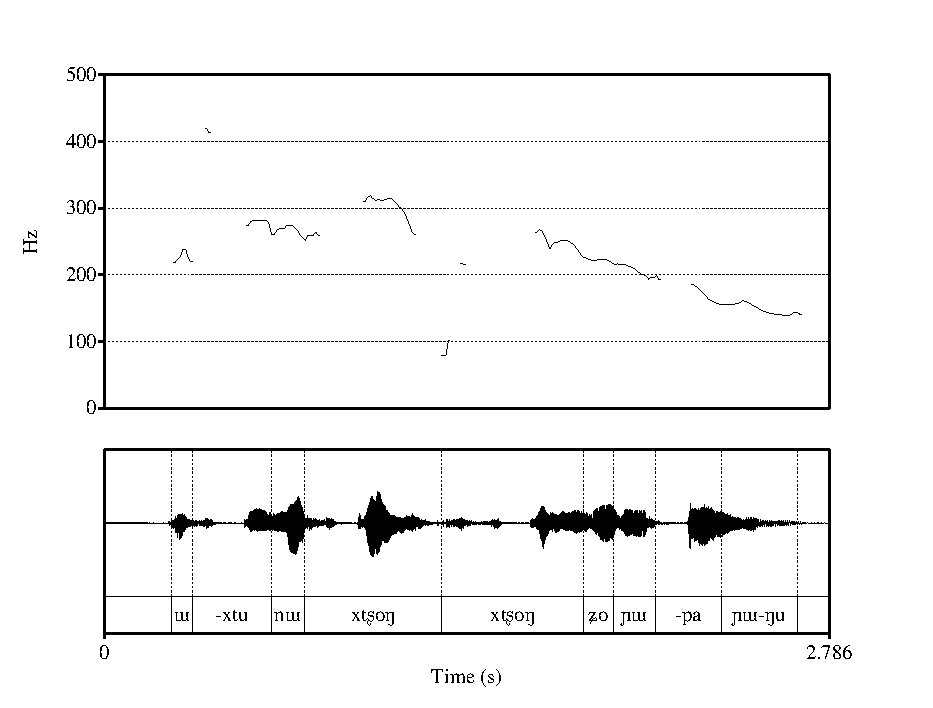
\includegraphics[width=\textwidth]{xtsxoN.eps}
\end{figure}

This emphatic pronunciation is not uncommon, but in most cases the ideophones do not have any special intonation. Example (§\ref{sec:xtsxoNxtsxoN2}) illustrates the same ideophone \forme{xtʂoŋxtʂoŋ} a few sentence later in the same text, without any emphasis.

\begin{exe}
\ex \label{sec:xtsxoNxtsxoN2}
\gll tɕe ma nɯnɯ tu-fka xtʂoŋxtʂoŋ ʑo ŋu. \\
\textsc{lnk} \textsc{lnk} \textsc{dem} \textsc{ipfv}-be.full \textsc{idph}(II):bloated \textsc{emph} be:\textsc{full} \\
\glt `[The tick] is full [from having drunk blood] and bloated.' (25-xCelwi)
\japhdoi{0003664\#S57}
\end{exe}

\subsection{The genesis of ideophones} \label{sec:genesis.idph}
While it cannot be \textit{a priori} excluded that some ideophones could be ancient, their phonological markedness is a sign that they are constantly renewed, using processes different from those found in non-ideophonic words. In this section, I propose a scenario account for one of the origins of ideophonic roots, and  ideophonic hybridization (§\ref{sec:idph.gradation}).

Some ideophonic roots are obviously built from Tibetan loanwords, but with slight phonetic changes. The most obvious case is \idroot{ldʑɯŋ} `skyblue', which originates from the first syllable of \tibet{ལྗང་ཁུ་}{ldʑaŋ.kʰu}{green} (also borrowed as the unpossessible noun \japhug{ldʑaŋkɯ}{blue/green}, §\ref{sec:tibetan.colours}) with a slight modification of the vowel. The semantic relationship between the ideophone and the Tibetan borrowing is not always as obvious. For instance, \idroot{zɟaŋ} and \idroot{zɟraŋ}, both meaning `filled up, looking soft' (of a person's belly, a bag filled with objects) are reminiscent of the verb \japhug{βrɟaŋ}{stretch tight} (of skin), which is borrowed from the past tense of \tibet{རྒྱོང་བརྒྱངས་}{rgʲoŋ.brgʲaŋs}{stretch, distend}: the ideophones describe a skin or membrane that is overstretched and distended, like the result of the action expressed by the verb \forme{βrɟaŋ}. The form \idroot{zɟaŋ} could either have been independently borrowed from a Tibetan variety where \forme{r-} and \forme{s-} merge, or directly based on \forme{βrɟaŋ} with further consonant modification. The root \idroot{zɟraŋ} is derived from \idroot{zɟaŋ} by insertion of \forme{-r-} (see below for a possible account of these sporadic sound changes).
 
The Tibetan origin of some ideophones is one possible reason for the frequency of voiced stops in ideophones (§\ref{sec:idph.onsets}), as \ipa{b}, \ipa{d}, \ipa{ɟ} and \ipa{g} are common in clusters in the borrowed layer.

However, in many case the lexical origin of ideophones has been completely blurred by a variety of mechanisms which can only be hypothesized. The four synonymous ideophones \forme{dzoʁ} (\ref{ex:dzoR.Zo.pjAtshoR}), \forme{zgoʁ}, \forme{goʁ} and \forme{dzɯr} (\ref{ex:dzWr.Zo.tanWtshoR}) exclusively occur in collocation with the transitive verb \japhug{tsʰoʁ}{attach} and the noun \japhug{tɯ-χpɯm}{knee} (§\ref{sec:tshoR.lv}) to express both the speed of the kneeling motion and the highly deferential attitude of the kneeling person.  

\begin{exe}
\ex \label{ex:dzoR.Zo.pjAtshoR}
\gll ɯ-χpɯm dzoʁ ʑo pjɤ-tsʰoʁ \\
\textsc{3sg}.\textsc{poss}-knee \textsc{idph}(I):kneeling \textsc{emph} \textsc{ifr}-attach \\
\glt `[The demon] immediately knelt down.' (140513 abide he mogui-zh) \japhdoi{0003975\#S45}
\end{exe}

\begin{exe}
\ex \label{ex:dzWr.Zo.tanWtshoR}
\gll ɯ-χpɯm dzɯr ʑo ta-nɯ-tsʰoʁ ndɤre, tɤ-lu pa-nɯ-tɕɤt ɲɯ-ŋu \\
 \textsc{3sg}.\textsc{poss}-knee \textsc{idph}(I):kneeling \textsc{emph} \textsc{aor}:3$'$\fl{}3-\textsc{auto}-attach \textsc{lnk} \textsc{indef}.\textsc{poss}-milk \textsc{aor}:3$'$\fl{}3-\textsc{auto}-take.out \textsc{sens}-be \\
 \glt `She immediately knelt down and milked [the cow].' (2003 Kunbzang)
\end{exe}

In addition to pattern I, they also occur in pattern III as in (\ref{ex:zgoRnAzgoR.Zo.tatshoRnW}).

\begin{exe}
\ex \label{ex:zgoRnAzgoR.Zo.tatshoRnW}
\gll  tɤ-pɤtso ra dɯxpa-nɯ matɕi tɕendɤre, zgoʁnɤzgoʁ ʑo nɯ-χpɯm ta-tsʰoʁ-nɯ tɕe \\
\textsc{indef}.\textsc{poss}-child \textsc{pl} poor-\textsc{pl} because \textsc{lnk} \textsc{idph}(II):kneeling \textsc{emph}  \textsc{3pl}.\textsc{poss}-knee \textsc{aor}:3$'$\fl{}3-attach-\textsc{pl} \textsc{lnk} \\
\glt `The poor children, they knelt [before the ogre] one after the other.' (160704 poucet4-v2)
\japhdoi{0006097\#S23}
\end{exe}

I propose that one of the mechanism of ideophone creation is by playful reanalysis from lexical verb roots. The four ideophones \forme{dzoʁ}, \forme{zgoʁ}, \forme{goʁ} and \forme{dzɯr}, which have either the onset \forme{(z)g-} or \forme{dz-} and the rhymes \forme{-oʁ} and \forme{-ɯr}, originate in my opinion from the verbs \japhug{ndzoʁ}{be attached} (the anticausative of \japhug{tsʰoʁ}{attach}, §\ref{sec:anticausative.dummy}) and \japhug{azgɯr}{bow, bend down} (the latter borrowed from \tibet{སྒུར་}{sgur}{bend down}). The development of these ideophones occurred in three steps, as illustrated in \figref{fig:idph.dzoR}.


\begin{figure}[H]
\caption{Development of the family of ideophones meaning `kneeling respectfully'} \label{fig:idph.dzoR}  
\begin{tikzpicture}
\node (A) at (-4,0) { \japhug{ndzoʁ}{be attached} };
\node (B) at (4,0) { \japhug{azgɯr}{bow, bend down} };
\node (C) at (-3,-1.5) {\forme{dzoʁ} };
\node (D) at (3,-1.5) {\forme{*zgɯr} };
\node (E) at (1,-3) {\forme{dzɯr} };
\node (F) at (-1,-3) {\forme{zgoʁ} };
\node (G) at (0,-4) {\forme{goʁ} };
\tikzstyle{direct}=[->,very thick,>=latex]
\tikzstyle{blend}=[->,dotted,very thick,>=latex]
\draw[direct] (A)--(C);
\draw[direct] (B)--(D);
\draw[blend] (D)--(F);
\draw[blend] (D)--(E);
\draw[blend] (C)--(E);
\draw[blend] (C)--(F);
\draw[direct] (F)--(G);
\end{tikzpicture}
\end{figure}

First, the ideophone roots \forme{dzoʁ} `kneeling' (with alternation to the more marked plain voiced \forme{dz-} onset, §\ref{sec:consonant.phonemes}) and an unattested \forme{*zgɯr} (perhaps `kneeling and bowing') were directly created from the two verbs. The forms \forme{zgoʁ} and \forme{dzɯr} result from blending from the two primary ideophones \forme{dzoʁ} and \forme{*zgɯr} by exchanging rhyme and onset. Third, \forme{goʁ} was derived from \forme{zgoʁ} by simplification of the onset.

This process is not a derivation in the proper sense, since it is neither regular nor predictable, and involves processes such as blending which do not normally occur in the verbal and nominal morphology of the Japhug language.

In addition to native roots and Tibetan loanwords, an obvious source of ideophones are onomatopoeic imitations of natural sounds. However, given the fact that ideophonic changes do not follow regular rules unlike the normal vocabulary on the one hand, and that northern Gyalrong languages lack historical records on the other hand, it is unlikely that the prehistory of this type of ideophones can be recovered.


\subsection{Syntax of ideophones} \label{sec:idph.syntax}
As pointed out by \citet[660]{dingemanse12ideo}, the markedness of ideophones is not limited to their phonology, but is also manifested in their syntactic behaviour.

Ideophones nearly always occur as verb adjuncts in Japhug. They are most commonly found with the intransitive light verb \forme{pa}, the quotative verb \japhug{ti}{say} and the similative verb \japhug{stu}{do like}, following a cross-linguistically well-attested pattern (\citealt[280--288]{guldemann08quot}). They can also be used as adjunct of any lexical verb in either nominalized or finite form, and in a handful of examples, as noun modifiers. Ideophones commonly occur with the emphatic \forme{ʑo} (§\ref{sec:emphatic.Zo}), which follows them.

%{sec:light.verb}
\subsubsection{The auxiliary \forme{pa}} \label{sec:idph.pa}
The intransitive verb \forme{pa} (also attested in collocation with numerals, §\ref{sec:pa.intr.lv}) is one of the most common light verb used with ideophones. It is the labile intransitive counterpart (§\ref{sec:lability.pass}) of the verb \japhug{pa}{do}, which also occurs as a light verb in noun-verb collocations (§\ref{sec:pa.lv}). 

It can either appear as an inflected form as in (\ref{ex:RYJli.Zo.YWpa}), or as the participle \forme{kɯ-pa} as in (\ref{ex:XploR.kWpa}) (see also \ref{ex:zjaNzjaN3}, §\ref{sec:ideo.II}). It is mainly used with pattern II ideophones describing colour, shape or spatial disposition.

 
\begin{exe}
\ex \label{ex:RYJli.Zo.YWpa}
\gll ɯ-pʰoŋbu nɯ rcanɯ ʁɲɟlíʁɲɟli ʑo ɲɯ-pa. \\
\textsc{3sg}.\textsc{poss}-body \textsc{dem} \textsc{unexp}:\textsc{deg} \textsc{idph}(II):huge \textsc{emph} \textsc{sens}-\textsc{aux} \\
\glt  `Its body, it is enormous.' (20-sWNgi) 	\japhdoi{0003562\#S16}
\end{exe}

\begin{exe}
\ex \label{ex:XploR.kWpa}
\gll aʑo grɯβgrɯβ ɯ-ftsa nɯ tɤ-kɯ-qawɤr ma nɯ ma χploʁχploʁ kɯ-pa mɯ-pɯ-mto-t-a \\
\textsc{1sg} matsutake \textsc{3sg}.\textsc{poss}-nephew \textsc{dem} \textsc{aor}-\textsc{sbj}:\textsc{pcp}-open.cap apart.from \textsc{dem} apart.from \textsc{idph}(II):small.and.spherical \textsc{sbj}:\textsc{pcp}-\textsc{aux} \textsc{neg}-\textsc{aor}-see-\textsc{pst}:\textsc{tr}-\textsc{1sg} \\
\glt `(The mushroom called) `the matsutake's nephew', I have seen ones with opened caps, but never seen one in ball shape (before the cap opens).' (23-grWBgrWBftsa)
\japhdoi{0003602\#S5}
\end{exe}

%{sec:xtsxoNxtsxoN}

Like other stative verbs, \forme{pa} has an inchoative meaning in the Imperfective (§\ref{sec:ipfv.inchoative}), the Aorist (§\ref{sec:aor.inchoative}) and the Inferential (§\ref{sec:ifr.inchoative}). It is attested with the \textsc{upwards} (\forme{tu-pa}, example \ref{ex:tupa.YWNu}) and the \textsc{westwards} (\forme{ɲɯ-pa}, example §\ref{sec:xtsxoNxtsxoN} in §\ref{sec:emphatic.idph}) orientation preverbs.


\begin{exe}
\ex \label{ex:tupa.YWNu}
\gll ɯ-ru nɯra nɯ-rom tɕe rʁɤβrʁɤβ tu-pa ɲɯ-ŋu  \\
\textsc{3sg}.\textsc{poss}-stalk \textsc{dem}:\textsc{pl} \textsc{aor}-dry \textsc{lnk} \textsc{idph}(II):rough \textsc{ipfv}-\textsc{aux} \textsc{sens}-be \\
\glt `Once it has dried, its stalk becomes very rough.' (14-sWNgWJu)
\japhdoi{0003506\#S21}
\end{exe}

While \forme{pa} is mainly found with pattern II ideophones, it is not restricted to these, and attested in a handful of examples with other patterns, such as III (\ref{ex:dWrnAdWr.pjApa}) and IV (\ref{ex:ckArnAlAr}).

\begin{exe}
\ex \label{ex:dWrnAdWr.pjApa}
\gll ʑɯrɯʑɤri qʰe li tɤ-se nɯ to-mbat qʰe, li tɤrmbɣo nɯ dɯrnɤdɯr pjɤ-pa \\
progressively \textsc{lnk} again \textsc{indef}.\textsc{poss}-blood \textsc{dem} \textsc{ifr}-diminish \textsc{lnk} again drum \textsc{dem} \textsc{idph}(III):drumming.far.away \textsc{ifr}.\textsc{ipfv}-\textsc{aux} \\
\glt `Progressively, the blood [in the lake] started to recede, and there was again a drumming sound far away.' (2003-kWBRa)
\end{exe}


\begin{exe}
\ex \label{ex:ckArnAlAr}
\gll ɕkɤrnɤlɤr ʑo kɯ-pa nɯ jo-nɯ-ɣi \\
\textsc{idph}(IV):limping \textsc{emph} \textsc{sbj}:\textsc{pcp}-\textsc{aux} \textsc{dem} \textsc{ifr}-\textsc{vert}-come \\
\glt `He came back home limping.' (140429 jiedi-zh)
\end{exe}

\subsubsection{Quotative \japhug{ti}{say}}\label{sec:idph.ti}
The verb \japhug{ti}{say} occurs as a light verb with ideophones expressing sound (\ref{ex:zJWG.Zo}, \ref{ex:tCRWz.nA.tCRWz}) and endopathic sensations (especially itching or pain as in \ref{ex:CYWG.Zo}), in patterns I (\ref{ex:zJWG.Zo}, \ref{ex:CYWG.Zo}), III (\ref{ex:tCRWz.nA.tCRWz}) and X (§\ref{sec:ideo.X}).

\begin{exe}
\ex \label{ex:zJWG.Zo}
\gll ɯ-tʰoʁ tɕu zɟɯɣ ʑo ti ɲɯ-ŋu\\
\textsc{3sg}.\textsc{poss}-ground \textsc{loc} \textsc{idph}(II):heavy.object.falling \textsc{emph} say:\textsc{fact} \textsc{sens}-be\\
\glt `[The stone] made a loud noise [as it fell] on the ground.' (2003 tWxtsa)
\end{exe}


\begin{exe}
\ex \label{ex:tCRWz.nA.tCRWz}
\gll cʰɯ-tɯt ɕɯŋgɯ tɕe tɕe tú-wɣ-ndza tɕe, tɕʁɯznɤtɕʁɯz tu-ti ɲɯ-ŋu tʰɯ-tɯt ɯ-qʰu tɕe tɕe tɤ́-wɣ-ndza tɕe, zwaʁnɤzwaʁ tu-ti ɲɯ-ŋu tɕe, nɯ ɲɯ-mɯm. \\
\textsc{ipfv}-be.ripe before \textsc{lnk} \textsc{lnk} \textsc{ipfv}-\textsc{inv}-eat \textsc{lnk} \textsc{idph}(III):crunchy.sound \textsc{ipfv}-say \textsc{sens}-be:\textsc{fact} \textsc{aor}-be.ripe \textsc{3sg}.\textsc{poss}-after \textsc{lnk} \textsc{lnk} \textsc{aor}-\textsc{inv}-eat \textsc{lnk} \textsc{idph}(III):not.crunchy \textsc{ipfv}-say \textsc{sens}-be \textsc{lnk} \textsc{dem} \textsc{sens}-be.tasty \\
\glt `If one eats [an apple]$_i$ before it$_i$ is ripe, it makes a crunchy sound, when it is ripe, it makes a soft (i.e. not crunchy) sound, it is [more] tasty (in this case because it has become sweeter and less sour).' (07-paXCi)
\japhdoi{0003430\#S22}
\end{exe}

\begin{exe}
\ex \label{ex:CYWG.Zo}
\gll tu-kɯ-ti kɯnɤ ɕɲɯɣ ʑo tu-ti tu-mŋɤm ŋu \\
\textsc{ipfv}-\textsc{genr}:S/O-say also \textsc{idph}(I):intense.pain \textsc{emph} \textsc{ipfv}-say \textsc{ipfv}-hurt be:\textsc{fact} \\
\glt `(When suffering from this disease), one feels intense pain even when one talks.' (29-RzAr)
\japhdoi{0003732\#S35}
\end{exe}


\subsubsection{The similative verb \japhug{stu}{do like} } \label{sec:stu.idph} 
The transitive similative verb \japhug{stu}{do like}  (§\ref{sec:ditransitive.secundative}, §\ref{sec:svc.similative.verb}) most commonly appears with the non-stative ideophonic patterns III (\ref{ex:lhWG.nA.lhWG})  and IV (\ref{ex:rloR.nA.rloR}). It expresses volitional actions, unlike \forme{pa} and \forme{ti}.  The syntactic function of the ideophones when used with \japhug{stu}{do like} is possibly that of semi-object, as they replace the demonstratives that usually occur with this verb (§\ref{sec:ditransitive.secundative}).

\begin{exe}
\ex \label{ex:lhWG.nA.lhWG}
\gll ɯ-sŋɯro lu-lɤt tɕe ɬɯɣnɤɬɯɣ, ɬɯɣnɤɬɯɣ tu-ste ɲɯ-ŋu.\\
\textsc{3sg}.\textsc{poss}-breath \textsc{ipfv}-release \textsc{lnk} \textsc{idph}(III):breathing.movement \textsc{idph}(III):breathing.movement \textsc{ipfv}-do.like[III] \textsc{sens}-be \\
\glt `When [the frog]$_i$ breathes, it$_i$ expands and retracts [its whole body] with each breath.' (27-qaCpa)
\japhdoi{0003716\#S3}
\end{exe}

The ideophone can describe the action as a whole (\ref{ex:lhWG.nA.lhWG}), or an aspect of the action on the object of \forme{stu} as in (\ref{ex:rloR.nA.rloR}), where the root \idroot{rloʁ}   depicts the shape of the fly's head (\tabref{tab:slaN.rloR}, §\ref{sec:idph.gradation}), and pattern III morphology (§\ref{sec:ideo.III}) the motion of the head.

\begin{exe}
\ex \label{ex:rloR.nA.rloR}
\gll ɯ-jaʁ tu-tsɯm tɕe, ɯ-ku ra pjɯ-nɯ-χtɕi tɕe ɯ-ku ra rloʁnɤrloʁ tu-ste ɲɯ-ŋu \\
\textsc{3sg}.\textsc{poss}-hand \textsc{ipfv}:\textsc{up}-take.away \textsc{lnk} \textsc{3sg}.\textsc{poss}-head \textsc{pl} \textsc{ipfv}-\textsc{auto}-wash \textsc{lnk} \textsc{3sg}.\textsc{poss}-head \textsc{pl}  \textsc{idph}(III):round  \textsc{ipfv}-do.like[III] \textsc{sens}-be \\ 
\glt `[The fly] stretches up its forelegs to clean its head (and the area around it), making (at the same time) a rhythmic rolling motion [with its head, round and minute].' (25-akWzgumba)
\japhdoi{0003632\#S46}
\end{exe}

The reflexive form \forme{ʑɣɤ-stu} (§\ref{sec:lexicalized.refl}) is almost exclusively attested with ideophones, in particular in the manner serial verb construction (§\ref{sec:svc.manner}) with other intransitive verbs, such as \forme{ku-rɤʑi} in (\ref{ex:XtshAXtshAt.Zo.tuZGAstu}). With pattern II ideophones, it means `make/have a $X$ look', generally expressing an attitude made on purpose.

 
\begin{exe}
\ex \label{ex:XtshAXtshAt.Zo.tuZGAstu}
\gll spɣi ɲɯ-nɯ-te ndɤre, nɤki rɟɤlpu tu-ɕe rcanɯ, tu-rɤjoʁβzɯr kɯ-fse rcanɯ, nɤki, χtsʰɤχtsʰɤt ʑo tu-ʑɣɤ-stu tɕe, ku-rɤʑi pɯ-ŋu, βdaʁmu tu-ɕe rcanɯ, pʰɤtɕʰɯχtɤr ʑo pjɯ-te tɕe, qɯqlɯ ʑo tu-ʑɣɤ-stu tɕe ku-rɤʑi pɯ-ŋu ɲɯ-ŋu. 	\\
attic \textsc{3sg}-inside \textsc{ipfv}:\textsc{east}-\textsc{auto}-put[III] \textsc{lnk} king  \textsc{ipfv}:\textsc{up}-go \textsc{unexp}:\textsc{deg} \textsc{ipfv}-clean.up \textsc{inf}:\textsc{stat}-be.like  \textsc{unexp}:\textsc{deg} \textsc{filler}  \textsc{idph}(II):lively.small \textsc{emph} \textsc{ipfv}-\textsc{refl}-do.like \textsc{lnk} \textsc{ipfv}-stay \textsc{pst}.\textsc{ipfv}-be  lady  \textsc{ipfv}:\textsc{up}-go  \textsc{unexp}:\textsc{deg} mess \textsc{emph} \textsc{ipfv}-put[III] \textsc{lnk} \textsc{idph}(II):hangdog.look \textsc{emph} \textsc{ipfv}-\textsc{refl}-do.like \textsc{lnk} \textsc{ipfv}-stay \textsc{pst}.\textsc{ipfv}-be \textsc{sens}-be \\
\glt `[The king]$_i$ put [the bird]$_j$ in the attic. When the king$_i$  would go up there, it$_j$ would clean everything up and would be lively; when the queen would go up there, it$_j$ would make a mess and have a hangdog look.' (2003 Kunbzang)
\end{exe}

It is also compatible with pattern I (\ref{ex:CNAB.Zo.tuZGAstu}) or III ideophones, expressing motion and/or sound.

\begin{exe}
\ex \label{ex:CNAB.Zo.tuZGAstu}
\gll tɕe nɯ kɯ-xtɕɯ\redp{}xtɕi ʑo ɲɯ́-wɣ-mbi tɕe ma ɕŋɤβ ʑo tu-ʑɣɤ-stu tɕe ju-nɯ-mɟe tɕe tu-ndze ɲɯ-ŋu. \\
\textsc{lnk} \textsc{dem} \textsc{sbj}:\textsc{pcp}-\textsc{emph}\redp{}be.small \textsc{emph} \textsc{ipfv}-\textsc{inv}-give \textsc{lnk} \textsc{lnk} \textsc{idph}(I):snapping \textsc{emph} \textsc{ipfv}-\textsc{refl}-do.like \textsc{lnk} \textsc{ipfv}-\textsc{auto}-take[III] \textsc{lnk} \textsc{ipfv}-eat[III] \textsc{sens}-be \\
\glt `We would give [our turtle]$_i$ a little piece$_j$ [of meat], and it$_i$ would grab it$_j$ with a snapping noise and eat it$_j$.' (140510 wugui)
\japhdoi{0003951\#S22}
\end{exe}

\subsubsection{Other verbs} \label{sec:ideophone.plus.lexical.verb}
Ideophones are not restricted in use to the light verbs cited above, and can appear with other types of verbs with compatible semantics. There are strict collocation restrictions, and most ideophones can only be used with one one or a handful of verbs. 

With the three light verbs discussed above (§\ref{sec:idph.pa}, §\ref{sec:idph.ti}, §\ref{sec:stu.idph}), ideophones are strictly preverbal, but when employed with other verbs, postverbal order is common, in particular in the case of stative adjectival verbs (\ref{ex:YWGWrni.tsGaRtsGaR}).

\begin{exe}
\ex \label{ex:YWGWrni.tsGaRtsGaR}
\gll ɯ-mɲaʁ wuma nɯ ɣɯ ɯ-rkɯ nɯra ɲɯ-ɣɯrni, ɲɯ-ɣɯrni tsɣaʁtsɣaʁ ʑo \\
\textsc{3sg}.\textsc{poss}-eye really \textsc{dem} \textsc{gen} \textsc{3sg}.\textsc{poss}-side \textsc{dem}:\textsc{pl} \textsc{sens}-be.red  \textsc{sens}-be.red \textsc{idph}(II):brilliant.red \textsc{emph} \\
 \glt `The sides of its eye proper are red, brilliant red.'  (23-qapGAmtWmtW) 	\japhdoi{0003608\#S47}
 \end{exe}

Ideophones can be postverbal even in particpial and finite relative clauses (§\ref{sec:relative.postverbal}), and can be located loser to the verb than determiners such as the indefinite \forme{ci} (§\ref{sec:indef.article}), as in (\ref{ex:kWGWrni.tsGaRtsGaR}).

 \begin{exe}
\ex \label{ex:kWGWrni.tsGaRtsGaR}
\gll [kɯ-ɣɯrni ʑo tsɣaʁtsɣaʁ] ci ŋu tɕe \\
\textsc{sbj}:\textsc{pcp}-be.red \textsc{emph} \textsc{idph}(II):brilliant.red \textsc{indef} be:\textsc{fact} \textsc{lnk} \\
\glt `[This species of millipede] is brilliant red.' (28-kWpAz)
\japhdoi{0003714\#S139}
   \end{exe} 
   
 When their semantic scope is more focalized on one of the arguments, the ideophone can directly follow a noun as in (\ref{ex:bAbAB.Zo.kundzoR}) or (\ref{ex:brWGbrWG.Zo.tutCAt}).

\begin{exe}
\ex \label{ex:bAbAB.Zo.kundzoR}
\gll tɯ-ŋga ɯ-taʁ ra ɯ-mat bɤbɤβ ʑo ku-ndzoʁ. \\
\textsc{genr}.\textsc{poss}-clothes \textsc{3sg}-on \textsc{pl}  \textsc{3sg}.\textsc{poss}-fruit \textsc{idph}(II):clumping.together \textsc{emph} \textsc{ipfv}-\textsc{acaus}:attach \\
\glt `When one walks among [these plants], their seeds attach in clumps to one's clothes.' (18-qromJoR)
\japhdoi{0003532\#S159}
\end{exe}

\begin{exe}
\ex \label{ex:brWGbrWG.Zo.tutCAt}
\gll rtɕʰɯʁjɯ ɣɯ ɯ-rme nɯ kɯ ɲɯ-kɯ-z-rɤʑa. nɯ tɯ-ɕa a-mɤ-nɯ-ɤtɯɣ ra ma tɤndɤr brɯɣbrɯɣ ʑo tu-tɕɤt ɲɯ-ŋu  \\
caterpillar \textsc{gen} \textsc{3sg}.\textsc{poss}-hair \textsc{dem} \textsc{erg} \textsc{ipfv}-\textsc{genr}:S/O-\textsc{caus}-itch \textsc{dem} \textsc{genr}.\textsc{poss}-flesh \textsc{irr}-\textsc{neg}-\textsc{pfv}-touch be.needed:\textsc{fact} \textsc{lnk} pimple \textsc{idph}(II):little.pimples \textsc{emph} \textsc{ipfv}-take.out \textsc{sens}-be \\
\glt `The caterpillar's hair itches people, it should not touch one's flesh, otherwise it will cause a lot of little pimples to appear.' (25-rtchWRjW)
\japhdoi{0003656\#S82}
\end{exe}
 
  
 \subsubsection{Noun modifier} \label{sec:ideophone.noun.modifier}
 In examples such as (\ref{ex:bAbAB.Zo.kundzoR}) or (\ref{ex:brWGbrWG.Zo.tutCAt}) (§\ref{sec:ideophone.plus.lexical.verb}), the syntactic status of the ideophone is ambiguous between a sentential adverb and a postnominal modifier. 
 
 Examples (\ref{ex:zJAGzJAG.ma}) and (\ref{ex:ndzArndzAr.ma}) are incontrovertible evidence that ideophones can serve as noun modifier: in (\ref{ex:zJAGzJAG.ma}) is embedded within an exceptive (§\ref{sec:exceptive}) postpositional phrase which does not contain any verb, and must be analyzed as modifier of the counted noun \forme{tɯ-rdoʁ} `one piece'.
 
\begin{exe}
\ex \label{ex:zJAGzJAG.ma}
\gll ma nɯnɯ ɕawurambɯm tu-ti-nɯ tɕe nɯnɯ, nɤkinɯ, [[tɯ-rdoʁ ʑo \textbf{zɟɤɣzɟɤɣ}] ma] kɯ-me ɲɯ-ŋu kʰi \\
\textsc{lnk} \textsc{dem} Shwa.ba.rwa.mbum \textsc{ipfv}-say-\textsc{pl} \textsc{lnk} \textsc{dem} \textsc{filler} one-piece \textsc{emph} \textsc{idph}(II):short.and.thick apart.from \textsc{sbj}:\textsc{pcp}-not.exist \textsc{sens}-be \textsc{hearsay} \\
\glt `People call it `Shwaba rwa'bum', it is [a kind of deer antler] with only one [branch], short and thick.'   (27-qartshaz) \japhdoi{0003702\#S72}
\end{exe}

In (\ref{ex:ndzArndzAr.ma}), the ideophone \forme{ndzɤrndzɤr} is in the emphatic exceptive construction, with the linker \forme{ma} (§\ref{sec:exceptive}).

\begin{exe}
\ex \label{ex:ndzArndzAr.ma}
\gll  <donglang> ɯʑo-sti nɯnɯ, [tɤ-tɕɯ tɯ-rdoʁ ndzɤrndzɤr] ma nɯ ma kɯ-tu pjɤ-me. \\
\textsc{anthr} \textsc{3sg}-alone \textsc{dem} \textsc{indef}.\textsc{poss}-son one-piece \textsc{idph}(II):alone \textsc{lnk} \textsc{dem} apart.from \textsc{sbj}:\textsc{pcp}-exist \textsc{ifr}.\textsc{ipfv}-not.exist \\
\glt `There remained only Donglang, the boy, all alone (on earth after his family had been taken away).' (150828 donglang)
\japhdoi{0006312\#S129}
\end{exe}

However, ideophones as postnominal modifiers are rare, and only occur in combination with a singular counted noun such as \forme{tɯ-rdoʁ} in the meaning `alone'. 
%For this reason, in examples such as (\ref{ex:bAbAB.Zo.kundzoR}) or (\ref{ex:brWGbrWG.Zo.tutCAt}) (§\ref{sec:ideophone.plus.lexical.verb}), ideophones are preferentially analyzed as sentential markers rather than noun modifiers.

\subsection{Discourse function}
 Ideophones are non-essential to communication in the sense that any sentence containing an ideophone can be glossed with another sentence of identical truth value without using any ideophone. The frequency of ideophones and ideophonic verbs presents considerable variation  in the corpus: some stories and procedural texts are almost devoid of them, while some episodes of traditional narratives are densely packed with them.
  
Ideophones convey rich and intricate meanings in a succinct way. In traditional stories, their use contributes to the vividness of the description. For instance, in  (\ref{ex:ndArndAr}), the choice of the pattern II \forme{ndɤrndɤr} `huge and imposing'	and 	the pattern III \forme{ɲcɣɤnɤɲcɣɤt} `loud and moving around' evokes  a much more expressive picture than the  translation provided here in plain language. Native speakers, upon hearing such a sentence, visualize the vivid picture of huge lush trees and flocks of birds flying around, tweeting and chirping.

\begin{exe}
\ex \label{ex:ndArndAr}
 \gll nɯra tɤ-stu-t-a tɕe,  sɯŋgɯnaχtɕɯn \textbf{ndɤrndɤr} ʑo nɯ-stu-t-a, ɯ-taʁ,  pɣa \textbf{ɲcɣɤnɤɲcɣɤt} ʑo ɲɯ-mbri tɕe \\
\textsc{dem}:\textsc{pl} \textsc{aor}-do.like-\textsc{pst}:\textsc{tr}-\textsc{1sg} \textsc{lnk} deep.forest \textsc{idph}(II):huge \textsc{emph} \textsc{aor}-do.like-\textsc{pst}:\textsc{tr}-\textsc{1sg} \textsc{3sg}-on birds \textsc{idph}(III):loud \textsc{emph} \textsc{sens}-call \textsc{lnk} \\
\glt `I acted this way, I created a huge and deep forest on the top of whose trees birds are tweeting and chirping and flying around.' (2011-04-smanmi)
\end{exe}


\section{Other expressive words} \label{sec:other.expressive}
Two classes of words present common properties with, but are different from, real ideophones: interjections (§\ref{sec:interjections}) and calling sounds (§\ref{sec:call}). Although both also present phonological markedness and some degree of iconicity, they are not subject to ideophonic morphology (§\ref{sec:ideo:morpho}) and do not share the same syntactic properties. 

In addition, we find some nouns which, unlike deideophonic verbs (§\ref{sec:GA.sA.deidph}), ideophonic counted nouns (§\ref{sec:CN.ideophones}) and nominal ideophonic compounds (§\ref{sec.n.idph.compounds}), are directly built on an expressive root without derivational morphology (§\ref{sec:underived.expressive.nouns}).

 
\subsection{Interjections} \label{sec:interjections}
 Interjections are marked words expressing a feeling or an emotion like ideophones, but differ from them in that they cannot serve as verb adjuncts, cannot receive ideophonic morphology and are mainly used in isolation, either in their own clause or as the reported speech complements of verbs of speaking like \japhug{ti}{say} (\ref{ex:atsatsa}, \ref{ex:wudzWdzi}). 
 
\begin{exe}
\ex \label{ex:atsatsa}
\gll tɤ-ɣɤndʐo tɕe `ɯtɕʰɯtɕʰɯ' ma-tɯ-ti, tɤ-sɤɕke tɕe (nɤkinɯ) `atsatsa' ma-tɯ-ti, kɯ-mŋɤm tɤ-tu tɕe `atsatsa' ma-tɯ-ti ra  \\
 	\textsc{aor}-be.cold \textsc{lnk} \textsc{interj}:cold \textsc{neg}:\textsc{imp}-2-say \textsc{aor}-\textsc{prop}-burn \textsc{lnk} \textsc{filler} \textsc{interj}:pain \textsc{neg}:\textsc{imp}-2-say \textsc{sbj}:\textsc{pcp}-hurt \textsc{aor}-exist \textsc{lnk} \textsc{interj}:pain \textsc{neg}:\textsc{imp}-2-say be.needed:\textsc{fact} 	\\
\glt `When you feel cold, don't say ``Ah'', when you feel hot, don't say ``ouch'', when you  feel pain, don't say ``ouch''.' (07-deluge) \japhdoi{0003426\#S64}
\end{exe}

\begin{exe}
\ex \label{ex:wudzWdzi}
\gll srɯtpʰu srɯnmɯ kɯ-fse kɯ-sɤ-ɣmɯ\redp{}ɣmu ʑo ɲɤ-k-ɤtɯɣ-ndʑi-ci ri,  `wudzɯdzi' mɯ-to-ti. \\
râkshasa râkshasî \textsc{sbj}:\textsc{pcp}-be.like \textsc{sbj}:\textsc{pcp}-\textsc{prop}-\textsc{emph}\redp{}fear \textsc{emph} \textsc{ifr}-\textsc{peg}-meet-\textsc{du}-\textsc{peg} \textsc{lnk} \textsc{interj}:fear \textsc{neg}-\textsc{ifr}-say \\
\glt `They met fearsome râkshasas and râkshasîs, but he did not say `how frightful!'.' (31-deluge) 	\japhdoi{0004077\#S114}
\end{exe}
 

Interjections can however be followed by full clauses, but with a pause as in (\ref{ex:aCi}) (see also for instance \forme{ja} in example \ref{ex:thWnWmblWmnW.je}, §\ref{sec:reported.speech.sfp}).

\begin{exe}
\ex \label{ex:aCi}
\gll aɕi! ɲɯ-tɯ-ɣɤŋgi.  \\
\textsc{interj}:correction \textsc{sens}-2-be.right \\
\glt `Of course (I take back what I have said)! You are right.' (2003 tWxtsa)
\end{exe} 


The marker \forme{wo} can precede without pause a noun in vocative function (\ref{ex:wo.amu}) (see also \ref{ex:pGAlnApGAl}, §\ref{sec:ideo.III}).
  
\begin{exe}
\ex \label{ex:wo.amu}
\gll wo a-mu a-kɯm ɣɯ-tɤ-ci  \\
\textsc{interj} \textsc{1sg}.\textsc{poss}-mother  \textsc{1sg}.\textsc{poss}-door \textsc{cisl}-\textsc{imp}-open[III] \\
\glt `Mother, come and open the door for me!' (2012 tWJo) 	\japhdoi{0004089\#S21}
\end{exe} 

Some interjections cannot form a complete utterance on their own:  \japhug{χawo}{if only} introduces a clause in the Irrealis expressing a wish (see examples \ref{ex:apWsatnW.YWsWsama}, §\ref {sec:irrealis.complement.clauses} and \ref{ex:atWrme}, §\ref{sec:frozen.indef}). The form \forme{tsatsatsa} is used in a correlative construction meaning  `one can say that $X$, but one can also say that $\neg X$, with the positive $X$ and negative $\neg X$ forms of the same verb followed by the additive \forme{nɤ}, as in (\ref{ex:tsatsatsa}).

\begin{exe}
\ex \label{ex:tsatsatsa}
\gll ɲɯ-tɯ-fse nɤ tsatsatsa, mɯ́j-tɯ-fse nɤ tsatsatsa \\
\textsc{sens}-2-be.like \textsc{add} \textsc{interj} \textsc{neg}:\textsc{sens}-2-be.like \textsc{add} \textsc{interj} \\
\glt  `One can say that you look like her, but one can also say that you don't.' (2014-kWlAG)
\end{exe}



Interjections can be classified into four categories (\tabref{tab:interjections}): involuntary responses to stimuli (interjections in the proper sense, \citealt{dingemanse11phd}), and uninflected words expressing comments on words uttered by oneself or others, short orders or polite expressions.
  
\begin{table}[t]
\caption{List of interjections} \label{tab:interjections}
\begin{tabular}{lll}
\lsptoprule
Category &Form & Function \\
\midrule
Involuntary  &\forme{ɯtɕʰɯtɕʰɯ}, \forme{wutɕʰɯtɕʰɯ} &  expresses cold \\  
response&\forme{atsatsa} &  expresses pain \\
&\forme{atsatsa} &  expresses pain \\
&\forme{wudzɯdzi} &  expresses fear \\
&\forme{ama}, \forme{amaŋ}  & expresses  surprise \\
&\forme{mtsʰɤri} & expresses  surprise \\
\midrule
Comment&\forme{aɕi} & taking back what one\\
&& has just said \\
&\forme{χawo} $X$ & `If only $X$' \\
&$X$\forme{tsatsatsa} $\neg X$\forme{tsatsatsa} & `One can say that $X$, but \\
&& one can also say that $\neg X$' \\
&\forme{maχtɕɯ} & `I told you so!' \\
&\forme{ɕaʁja} & `It serves you right!' \\
&\forme{woja} & confirmation \\
\midrule
Orders&\forme{cʰe},  \forme{pɤkʰije}& `wait!' \\
&\forme{kɯz} & `go!' \\
&\forme{ja} & `come on' \\
&&speech filler (§\ref{sec:fillers}) \\
\midrule
Phatic&\forme{kʰɤβzaŋ} & `here I am' \\
&\forme{kʰatʂu} & `thanks' \\
&\forme{wortɕʰi (wojɤr)} & `please' \\
&\forme{ɣa} & `yes' \\
&\forme{wowe} & response to words meaning `goodbye' \\
&\forme{woja} & confirmation \\
\lspbottomrule
\end{tabular}
\end{table}
 
Among these forms,  \japhug{pɤkʰije}{wait} is the only one with a clear internal etymology (from \forme{pɤjkʰu je}, §\ref{sec:tense.aspect.adverbs}). Some interjections are from Tibetan, including the polite expressions and \japhug{mtsʰɤri}{how strange} (§\ref{sec:mirative}), which is originally a uniflected predicate borrowed from  \tibet{མཚར་}{mtsʰar}{feel strange}.

Although interjections lack morphological alternation, the additive \forme{nɤ} can be inserted within \forme{wortɕʰi wojɤr} (which is borrowed from \tibet{འོར་ཆེ་}{ɦor.tɕʰe}{thanks}) to express repeated action as in (\ref{ex:wortChi.nA.wojAr}) (see also \ref{ex:wojAr.ntsW.toti}, §\ref{sec:tense.aspect.adverbs}), a use reminiscent of the Ideophonic patterns III (§\ref{sec:ideo.III}) and IV (§\ref{sec:ideo.IV})

 \begin{exe}
\ex \label{ex:wortChi.nA.wojAr}
\gll tɤ-tɕɯ nɯ kɯ ``wortɕʰi nɤ wojɤr ʑo" to-ti ɲɯ-ŋu \\
\textsc{indef}.\textsc{poss}-boy \textsc{dem} \textsc{erg} please \textsc{add} please \textsc{emph} \textsc{ifr}-say \textsc{sens}-be \\
\glt `The boy said `please' several times.' (qachGa 2012)
\japhdoi{0004087\#S79}
\end{exe}

The phatic expressions and \japhug{sɤrma}{good night} and \japhug{kɤnɤβdi}{take care}, though originally non-inflecting, can take number indexation suffixes (§\ref{sec:phatic.inflectionalization}) and have become quasi-verbs, though they are highly anomalous and defective. The interjection \forme{woːwe} can be used as a response to these expressions.

The expression \forme{kʰɤβzaŋ} `here I am' is uttered by the guest when he arrives at someone else's home; the hosts invites the guest inside by saying \forme{nɤ-tʂu} `your way'.

The interjection \forme{woja} `yes, right' occurs to confirm the validity of a previous statement, sometimes assertive as in (\ref{ex:woja.nW.kWfse}) but also with interrogative markers such as \forme{ɣe} (see \ref{ex:totsu.Ge}, §\ref{sec:fsp.interrog}). It can be used whether the addressee had a vocal reaction or not.

\begin{exe}
\ex \label{ex:woja.nW.kWfse}
\gll ɯnɯnɯ tɕendi <wazi> nɯ ɯ-mdoʁ wuma ʑo ɲɯ-ɤsɯ-ndo. woja, nɯnɯ kɯ-fse ɲɯ-ŋu. \\
\textsc{dem} west socks \textsc{dem} \textsc{3sg}.\textsc{poss}-colour really \textsc{emph} \textsc{sens}-\textsc{prog}-take \textsc{interj} \textsc{dem} \textsc{sbj}:\textsc{pcp}-be.like \textsc{sens}-be \\
\glt `It has the colour of the socks over there. Yes, it is like that.' (23-grWBgrWBftsa)
\japhdoi{0003602\#S44}
\end{exe} 


\subsection{Calling  and chasing sounds} \label{sec:call}
Calling and chasing sounds, also referred to as `summons' and `dispersals' (\citealt[318--319]{aikhenvald10imperative}) are sounds used by people to interact with animals.\footnote{French has the more colorful term \textit{huchement de berger} to designate this class of utterances.} They are used either to incite the animals to come forward in the direction of the speaker (calling sounds, as in \ref{ex:tCitCi3}) or to advance or go away (chasing sounds, as in \ref{ex:tCha.lWlu}). 

\begin{exe}
\ex 
\begin{xlist}
\ex \label{ex:tCitCi3}
\gll lɯlu ɲɯ́-wɣ-nɯ-ɤkʰɤzŋga qʰe {tɕítɕi tɕítɕi tɕítɕi} nɯra tu-kɯ-ti qʰe ju-ɣi ŋu \\
cat \textsc{ipfv}-\textsc{inv}-\textsc{appl}-shout \textsc{lnk} \textsc{call}:cat \textsc{dem}:\textsc{pl} \textsc{ipfv}-\textsc{genr}-say \textsc{lnk} \textsc{ipfv}-come be:\textsc{fact} \\
\glt `When one calls a cat, one says \forme{tɕítɕi tɕítɕi tɕítɕi} and it comes.' (06-huchements1)
\ex \label{ex:tCha.lWlu}
\gll lɯlu jú-wɣ-no tɕe ``tɕʰa" tu-kɯ-ti ŋu \\
cat \textsc{ipfv}-\textsc{inv}-chase \textsc{lnk} \textsc{chase}:cat \textsc{ipfv}-\textsc{genr}-say be:\textsc{fact} \\
\glt `When one chases a cat, one says \forme{tɕʰa}.' (06-huchements2)
\end{xlist}
\end{exe}

In Japhug, nearly all farm animals and pets, whether mammals or birds, have special dedicated calling sounds, a list of which is provided in \tabref{tab:calling.sounds}. In addition, a click sound for which no IPA symbol exists is used to call puppies.

\begin{table}
\caption{Calling and chasing sounds in Japhug} \label{tab:calling.sounds}
\begin{tabular}{lllll}
\lsptoprule
 & 	animal & 	order \\ 	
 \midrule
\forme{tɕʰa} & 	\japhug{lɯlu}{cat} & 	chasing \\ 	
\forme{tɕítɕi tɕítɕi tɕítɕi} & 	  & 	calling \\ 	
 \midrule
\forme{wɯle} & 		\japhug{nɯŋa}{cow} & 	chasing \\ 	
\forme{aβleβle} & 	  & 	calling \\ 	
 \midrule
\forme{buwo} & 	\japhug{mbala}{bull} & 	chasing \\ 	
\forme{abobo} & 	  &  calling \\ 	
 \midrule
\forme{tsaʔ tsaʔ}, \forme{tsotsa} &  \japhug{kʰɯna}{dog} & 	calling \\ 	
\forme{soŋ} & 	 & 	chasing \\ 	
 \midrule
\forme{tʂutʂutʂutʂutʂutʂu} & 	\japhug{kumpɣa}{fowl} & 	calling \\ 	
\forme{kɕɯt} &   & 	chasing \\ 	
 \midrule
\forme{χaj} & 	\japhug{mbro}{horse} & 	chasing \\ 	
\forme{a̤ a̤ a̤ a̤} & 	 & 	calling \\ 	
 \midrule
\forme{zʁozʁozʁozʁo} & 	\japhug{ftsoʁ}{female hybrid yak} & 	calling \\ 	
\forme{acʰocʰo} & 	\japhug{jla}{male hybrid yak} & 	calling \\ 	
 \midrule
\forme{tɕʰɤt} & 	\japhug{paʁ}{pig} & 	chasing \\ 	
\forme{anininini, ʔwan, ʔwan ʔwan} & 	pig (adult) & 	calling \\ 	
\forme{anininini ǀǀǀǀǀǀ} & 	pig (little) & 	calling \\ 	
 \midrule
\forme{alolo} & 	\japhug{qaʑo}{sheep}  & 	calling \\ 	
\forme{titititi} & 	\japhug{tsʰɤt}{goat}  & 	calling \\ 	
\forme{kʰɯɕɯ} & 	goat, sheep & 	chasing \\ 	
\lspbottomrule
\end{tabular}
\end{table}

Given the rudimentary nature of man-animal interactions, it is not surprising that these sounds cannot be subjected to any morphological  operation other than reduplication. They cannot be used with any light verbs or occur as adjuncts. However, if the animal has a name, it can be added after the calling/chasing sound (\ref{ex:aBleBle.rgWskW}).

\begin{exe}
\ex \label{ex:aBleBle.rgWskW}
\gll tɕe ɯʑo kɯ-ɤskɯ a-pɯ-ŋu qʰe ``aβleβle rgɯskɯ" tu-kɯ-ti qʰe tɕe ɯʑo tso ɕti qʰe ju-nɯ-ɣi ɕti \\
\textsc{lnk} \textsc{3sg} \textsc{sbj}:\textsc{pcp}-having.white.colour.on.the.back \textsc{irr}-\textsc{ipfv}-be \textsc{lnk} \textsc{calling}:cow cow.name \textsc{ipfv}-\textsc{genr}-say \textsc{lnk} \textsc{lnk} \textsc{3sg} understand:\textsc{fact} be.\textsc{aff}:\textsc{fact} \textsc{lnk} \textsc{ipfv}-\textsc{auto}-come be.\textsc{aff}:\textsc{fact} \\
\glt `If [the cow] has white colour on the back (and is given the name \forme{rgɯskɯ}), one says \forme{aβleβle rgɯskɯ} and she understands, and comes by herself.' (06-huchements1)
\end{exe}

Phonologically, these words contain very unusual sounds: they make use of consonants and vowel that are not found at all in the standard lexicon: the dental click  \ipa{ǀ}, the glottal stop in a cluster \ipa{ʔw} or as a coda and breathy voice.

Only one of these words appears to have an identifiable etymology: \forme{soŋ} `chasing sound for dogs' is possibly related to Tibetan \tibet{སོང་}{soŋ}{go}. However, there is a striking resemblance between some of the chasing/calling sounds in Japhug and  Khroskyabs (\citealt[227]{lai17khroskyabs}), as illustrated by \tabref{tab:calling.sounds.japhug.khroskyabs}. It is unlikely that these resemblances are due to common inheritance.


\begin{table}
\caption{Calling/chasing sounds in Japhug and Khroskyabs} \label{tab:calling.sounds.japhug.khroskyabs}
\begin{tabular}{lllll}
\lsptoprule
Japhug & Meaning &Khroskyabs & Meaning \\
 \midrule
\forme{aβleβle} & calling a cow & \forme{vlêːvlevle} & calling a hybrid yak \\ 	
\forme{tsaʔ tsaʔ} &calling a dog & \forme{tsâ} & calling a dog \\ 		
\forme{soŋ} &  chasing a dog & \forme{sʊ̂ŋ} & chasing a dog \\ 			
\forme{tʂutʂutʂutʂutʂutʂu} &  calling a fowl & \forme{tʂûːtʂutʂu} &calling a fowl\\ 	
\lspbottomrule
\end{tabular}
\end{table}

\subsection{Deonomatopoeic expressive nouns} \label{sec:underived.expressive.nouns}
A certain number of bird names are based on onomatopoeia imitating their song. For instance, \japhug{qusput}{cuckoo}  (example \ref{ex:ntsW.tuti}, §\ref{sec:tense.aspect.adverbs})  and \japhug{tsɯʁot}{pheasant} (\ref{ex:tsWRot.tuti}) are described as making a sound identical to their Japhug name.

\begin{exe}
\ex \label{ex:tsWRot.tuti}
\gll  tsɯʁot pʰu nɯ tu-mbri tɕe, {``tsɯʁot tsɯʁot tsɯʁot"} ntsɯ tu-ti ŋu. \\
pheasant male \textsc{dem} \textsc{ipfv}-make.sound \textsc{lnk} \textsc{idph}(X):cry always \textsc{ipfv}-say  be:\textsc{fact} \\
\glt `When the male pheasant sings, it says \forme{tsɯʁot tsɯʁot tsɯʁot}.' (24-kWmu) 	\japhdoi{0003618\#S104}
\end{exe}

In the case of  \japhug{dɯdɯt}{turtle dove}, its calling sound is described as being slightly different from its name, with various interpretations (\ref{ex:dudut.tuti}).\footnote{In Tshobdun, `pheasant' and `turtle-dove' are called \forme{tsəʁot} and \forme{dudut}, respectively \citep[137]{jackson19tshobdun}. These words cannot be inherited from the common ancestor of Japhug and Tshobdun however, since Tshobdun \forme{-ot} should correspond to either \forme{-ɤt} or \forme{-ɯt}. }

\begin{exe}
\ex \label{ex:dudut.tuti}
\gll tɕe dɯdɯt kɤ-ti ci tu tɕe, tɕe {``dudut dudut"}  ntsɯ tu-ti. tsuku kɯ ``dudut cɯŋglɯɣ" tu-ti ŋu ra tu-ti-nɯ ri, nɯ mɤ-xsi ri, {``dudu wu"} kɯ-fse tu-ti ŋgrɤl. \\
\textsc{lnk} turtle.dove \textsc{obj}:\textsc{pcp}-say \textsc{indef} exist \textsc{lnk} \textsc{lnk} onomatopoeia always \textsc{ipfv}-say some \textsc{erg} onomatopoeia mortar \textsc{ipfv}-say  be:\textsc{fact} pl \textsc{ipfv}-say-\textsc{pl} \textsc{lnk} \textsc{dem} \textsc{neg}-\textsc{genr}:know \textsc{lnk} onomatopoeia \textsc{sbj}:\textsc{pcp}-be.like \textsc{ipfv}-say be.usually.the.case:\textsc{fact} \\
\glt `There is [a bird] called turtle-dove, it always makes \forme{dudut dudut}. Some people say that it makes \forme{dudut cɯŋglɯɣ}, I don't know [if it is true], [in any case] it makes \forme{dudut wu}.' (22-CAGpGa)
\japhdoi{0003586\#S24}
\end{exe}

The bird name \forme{tacoʁcoʁ} is based on the onomatopoeia describing its song (see example \ref{ex:tWrtsAG.tAmbro}, §\ref{sec:imp.function}), but with the addition of a \forme{ta-} prefix, which may or may not be related to the action nominal \forme{tɯ-} prefix (§\ref{sec:action.nominals}).

\section{Speech fillers} \label{sec:fillers}
In Japhug speech fillers, rather than a central vowel, are used to mark pause during speech either due to hesitation, or to give the speaker more time to reflect on what he or she is about to say.

The cataphoric demonstrative \forme{nɤki}, used both as a pronoun (§\ref{sec:cataph.pron}) and as a noun modifier (§\ref{sec:demonstrative.determiners}), is the most frequent speech filler (examples in this grammar include \ref{ex:YWwGrWwGrum} in §\ref{sec:emph.redp}, \ref{ex:tWNgo.ZimkhAm} in §\ref{sec:nominal.intensifier} and \ref{ex:lurYJi.tsa.Nu} in §\ref{sec:preverb.adjectives.size}). It can be combined with the determiner \forme{nɯ} (§\ref{sec:nW.topic}) as \forme{nɤkinɯ} (\ref{ex:pjAkAtaci.passive}, §\ref{sec:preverbs.contracting.verbs}) or with the indefinite \forme{ci} (§\ref{sec:indef.article}) as \forme{nɤki ci nɯ}. 
  
The aforementioned anaphoric topic marker \forme{iɕqʰa} (§\ref{sec:iCqha}), which derives from the adverb \japhug{iɕqʰa}{just now}, also occurs as speech filler (example \ref{ex:CkunWrtCe}, §\ref{sec:echo.multiple.AM}), likewise frequently followed by the determiner \forme{nɯ} (\ref{ex:WphWNgW.nWtCu.YAtCAt}, §\ref{sec:manipulation.verbs} and \ref{ex:CtuBzdWnW}, §\ref{sec:AM.goal}).


\begin{exe}
\ex \label{ex:nAkinW.iCqhanW}
\gll nɯnɯ tɕe, pɕi ku-rɤʑi ɕti tɕe, nɤki nɯ, iɕqʰa nɯ, kʰa ɯ-ŋgɯ ju-ɣi mɤ-ŋgrɤl \\
\textsc{dem} \textsc{lnk} outside \textsc{ipfv}-stay be.\textsc{aff}:\textsc{fact} \textsc{lnk} \textsc{filler} \textsc{dem} \textsc{filler} \textsc{dem} house \textsc{3sg}.\textsc{poss}-in \textsc{ipfv}-come \textsc{neg}-be.usually.the.case:\textsc{fact} \\
\glt `That one (the wild cat), it stays outside, it does not come inside houses (unlike the domestic cat).' (21-lWLU) 	\japhdoi{0003576\#S5}
\end{exe}

The interjection \forme{ja} (§\ref{sec:interjections}) is used as speech filler by persons listening to traditional stories, as a sign that they are following the narrative of the storyteller. Traditional storytellers require their audience to respond in this way, as shown by (\ref{ex:ja.tAti.ma.tCe}).

\begin{exe}
\ex \label{ex:ja.tAti.ma.tCe}
\gll ``ja" tɤ-ti ma tɕe mɯ́j-kʰɯ. \\
\textsc{filler} \textsc{imp}-say \textsc{lnk} \textsc{lnk} \textsc{neg}:\textsc{sens}-be.possible \\
\glt `Say `ya', otherwise [I] can't [tell the story].' (160720 kandZislama)
\japhdoi{0006147\#S3}
\end{exe}

\section{Sentence final particles} \label{sec:sfp}
Japhug has a rich system of sentence final particles, which combine with verbal morphology to express modality, evidentiality, interrogation and the attitude of the speaker.

Given the fact that the meaning of most sentence final particles is rather difficult to pinpoint with precision, the non-specific gloss \textsc{sfp} is used for all of them.
 
\subsection{Particles used in commands} \label{sec:fsp.imp}
The particle \forme{je} conveys a milder tone to orders expressed with Imperative (§\ref{sec:imperative}), Irrealis (§\ref{sec:irrealis}) and Prohibitive (§\ref{sec:prohibitive}), as shown by (\ref{ex:guan.makAtWBze}) (see also \ref{ex:jAlAt.je} in §\ref{sec:imp.function} and §\ref{sec:imp.autive} in §\ref{ex:tAnWndAm.je}).


\begin{exe}
\ex \label{ex:guan.makAtWBze}
\gll pɤkʰije tɕe <guan> ma-kɤ-tɯ-βze je! \\
wait \textsc{lnk} turn.off \textsc{neg}-\textsc{imp}-2-make[III] \textsc{sfp} \\
\glt `Wait, don't hang up [your phone].' (conversation, 2015-07-05)
\end{exe}

It combines with first person Imperfective verb forms to express hortative meaning (§\ref{sec:ipfv.hortative}) as in (\ref{ex:chWGia.je}). 

\begin{exe}
\ex \label{ex:chWGia.je}
\gll  aʑo cʰɯ-ɣi-a je ma mɤ-pʰan-a nɤ mɤ-ʁdɯɣ-a tʰaŋ nɤ \\
\textsc{1sg} \textsc{ipfv}:\textsc{downstream}-come-\textsc{1sg} \textsc{sfp} \textsc{lnk} \textsc{neg}:be.efficient:\textsc{fact}-\textsc{1sg} \textsc{add} \textsc{neg}-harm:\textsc{fact}-\textsc{1sg} \textsc{sfp} \textsc{sfp} \\
\glt `Let me come along, even if I am of no use, I will not do any harm.' (several occurrences)
\japhdoi{0003368\#S20}
\end{exe}

It is also used with 2\fl{}1 Imperfective forms to express  commands with a first person object as in (\ref{ex:pjWkWrkua.je}), since Imperative lacks 2\fl{}1 forms (§\ref{sec:imperative}).

\begin{exe}
\ex \label{ex:pjWkWrkua.je}
\gll a-wi tɕʰorzi ɯ-ŋgɯ pjɯ-kɯ-rku-a je\\
\textsc{1sg}.\textsc{poss}-grandmother jar \textsc{3sg}.\textsc{poss}-in \textsc{ipfv}:\textsc{down}-2\fl{}1-put.in-\textsc{1sg} \textsc{sfp}\\
\glt `Grandmother, put me in the jar, and...' (2005 Kunbzang)
\end{exe}

In addition, the particle \forme{je} is often added to phatic expressions such as \forme{tɤ-ɤstu} `goodbye', \japhug{sɤrma}{good night} and \japhug{kɤnɤβdi}{take care} (§\ref{sec:phatic.inflectionalization}) as in (\ref{ex:kAnABdi.je}).


\begin{exe}
\ex \label{ex:kAnABdi.je}
\gll kɤnɤβdi je a-mu! \\
take.care \textsc{sfp} \textsc{1sg}.\textsc{poss}-mother \\
\glt `Take care, mother!' (Gesar,54)
\end{exe}

Other postverbal elements used with Modal categories include the noun \japhug{smɯlɤm}{prayer} which occurs with the Irrealis (§\ref{sec:smWlAm.TAME}) and the softened command particle \forme{wo} (originally an interjection) as in (\ref{ex:nWBde.wo}). This particle can be cliticized to the verb stem (§\ref{sec:verb.enclitics}).

\begin{exe}
\ex \label{ex:nWBde.wo}
\gll  kʰu nɯ ʁo nɯ-βde wo, a-me nɯ χtanɤ a-ftsaʁ ɯβrɤ-ɣi ma \\
tiger \textsc{dem} \textsc{advers} \textsc{imp}-throw \textsc{sfp} \textsc{1sg}.\textsc{poss}-daughter \textsc{dem} \textsc{comp} \textsc{1sg}.\textsc{poss}-roof.leak \textsc{rh}.\textsc{q}-come \textsc{sfp} \\
\glt `My daughter, don't worry about the tiger, [I am more worried] that my [house] could have a roof leak.' (khu 2005)
\japhdoi{0004085\#S4}
\end{exe}

The \forme{je} and \forme{wo} particles are curiously similar to the Imperative and Hortative suffixes \forme{-(j)e} and \forme{-(w)ɵ} in the Kiranti language Khaling (\citealt[1114--1123]{jacques12khaling}), though it is extremely unlikely that this could reflect common inheritance, and is rather a pure coincidence.\footnote{In any case, Proto-Rgyalrong \forme{*-o} yields Japhug \forme{-u} (§\ref{sec:historical.phono}). }


\subsection{Particles used in polar questions} \label{sec:fsp.interrog}
In addition to the interrogative prefix \forme{ɯ-} (§\ref{sec:interrogative.W}), and interrogative pronouns (§\ref{sec:interrogative.pronouns}), questions can be marked by a series of several interrogative particles.

The particle \forme{ɕi} is the most common way of expressing a polar question, in combination with a verb in assertive form as in (\ref{ex:pjWmnata.Ci}) and (\ref{ex:nAZWB.WYWGi.Ci}). In this function, it is equivalent to the prefix \forme{ɯ-} (§\ref{sec:interrogative.W}).

\begin{exe}
\ex \label{ex:pjWmnata.Ci}
\gll kɯki li pjɯ-mnat-a ɕi? \\
\textsc{dem}.\textsc{prox} again \textsc{ipfv}-repeat-\textsc{1sg} \textsc{qu} \\
\glt `Do I tell [the story] again?' (150908 menglang-zh) \japhdoi{0006320\#S1}
\end{exe}

\begin{exe}
\ex \label{ex:nAZWB.WYWGi.Ci}
\gll nɤ-ʑɯβ ɲɯ-ɣi ɕi? \\
\textsc{2sg}.\textsc{poss}-sleep \textsc{sens}-come \textsc{qu} ? \\
\glt `Are you feeling sleepy?' (09-stoR,  65) \japhdoi{0003470\#S60}
\end{exe}

It can be used to express an alternative between two possibilities (\ref{ex:chWtWnWBlWnW.Ci}), often with an assertive verb form followed by the corresponding negative one (\ref{ex:YWmpCAr.Ci}).

\begin{exe}
\ex \label{ex:chWtWnWBlWnW.Ci}
\gll nɯʑora smi cʰɯ-tɯ-nɯ-βlɯ-nɯ ŋu ɕi, <dian> cʰɯ-tɯ-nɯmbjɯm-nɯ ŋu? \\
\textsc{2pl} fire \textsc{ipfv}-2-\textsc{auto}-burn-\textsc{pl} be:\textsc{fact} \textsc{qu} electricity \textsc{ipfv}-2-get.warm-\textsc{pl} be:\textsc{fact} \\
\glt `Do you burn a fire, or do you get warm with an electric [radiator]?' (conversation, 2013-12-13)
\end{exe}

\begin{exe}
\ex \label{ex:YWmpCAr.Ci}
\gll kɯki a-χpi ki ɲɯ-mpɕɤr ɕi mɯ́j-mpɕɤr? \\
\textsc{dem}.\textsc{prox} \textsc{1sg}.\textsc{poss}-story \textsc{dem}.\textsc{prox} \textsc{sens}-be.beautiful \textsc{qu} \textsc{neg}:\textsc{sens}-be.beautiful \\
\glt `Is this story of mine beautiful or not?' (140512 fushang he yaomo-zh)
\japhdoi{0003967\#S176}
\end{exe}

Furthermore, \forme{ɕi} can indicate a disjunction between more than two options. In this function, it is repeated after each clause in the disjunction, except the last one, as in (\ref{ex:tAnWmdzW.Ci}) (see also \ref{ex:tWnWCe.Ci}, §\ref{sec:disjunction.clauses}).

\begin{exe}
\ex \label{ex:tAnWmdzW.Ci}
\gll  χsɤr kʰri ɯ-taʁ tɯ-ɤ<nɯ>mdzɯ ɕi, rŋɯl kʰri ɯ-taʁ tɯ-ɤ<nɯ>mdzɯ ɕi, (...) ɕom kʰri ɯ-taʁ tɯ-ɤ<nɯ>mdzɯ ɕi, si kʰri ɯ-taʁ tɯ-ɤ<nɯ>mdzɯ? \\
gold seat \textsc{3sg}.\textsc{poss}-on 2-<\textsc{auto}>sit:\textsc{fact}  \textsc{qu} silver seat \textsc{3sg}.\textsc{poss}-on 2-<\textsc{auto}>sit:\textsc{fact}  \textsc{qu}  {  } iron seat \textsc{3sg}.\textsc{poss}-on 2-<\textsc{auto}>sit:\textsc{fact}  \textsc{qu} wood seat \textsc{3sg}.\textsc{poss}-on 2-<\textsc{auto}>sit:\textsc{fact}  \\
\glt `Will you sit on the golden seat, the silver seat, the iron seat or the wooden seat?' (2005 Kunbzang)
\end{exe}

The apprehensive prefix \forme{ɕɯ-} is likely to have been grammaticalized from this particle (§\ref{sec:apprehensive.history}).

The particle \forme{kɯ} occurs in questions to oneself (\ref{ex:nanWri.kW}), rhetorical questions and confirmation-seeking questions  (\ref{ex:future.GAZu}, §\ref{sec:sensory.functions}). Unlike \forme{ɕi}, it occurs together with either an interrogative pronoun or in combination with an interrogative verb form.\footnote{Example  (\ref{ex:nanWri.kW}) could be translated into French using the marker \textit{donc} as `Mais où est \textbf{donc} passé mon mendiant (de mari)?' } It is particularly common with the Dubitative (§\ref{sec:dubitative}).

\begin{exe}
\ex \label{ex:nanWri.kW}
\gll a-rcɤmbe-ŋga nɯ ŋotɕu nɯ-a<nɯ>ri kɯ? \\
\textsc{1sg}.\textsc{poss}-old.jacket-wear \textsc{dem} where \textsc{aor}:\textsc{west}-<\textsc{auto}>go[II] \textsc{qu} \\
\glt `Where did my beggar (`wearer of an old jacket") of a husband vanish?' (2005 Kunbzang)
\end{exe}

It can be combined with the particles \forme{ma}  (§\ref{sec:fsp.epistemic})  and \forme{ɣe} (see below) as \forme{kɯma} (\ref{ex:mWpWfCAttCi.kWma}) and \forme{kɯɣe}.

\begin{exe}
\ex \label{ex:mWpWfCAttCi.kWma}
\gll  mɤʑɯ tɕʰi mɯ-pɯ-fɕɤt-tɕi kɯma? \\
 even.more what \textsc{neg}-\textsc{aor}-tell-\textsc{1du} \textsc{qu} \\
 \glt `Which [trees] are there which we have not yet told [a story] about?' (13-tApWpjoR) 	\japhdoi{0003494\#S60}
\end{exe} 

Several particles mark a question inviting the addressee to confirm what the speaker has said: \forme{ɣe}, which even resembles an interjection in that it can be preceded by a pause as in (\ref{ex:totsu.Ge}), \forme{nétɕi} (\ref{ex:YWNu.netCi}, \ref{ex:totia.Nu.netCi}) and \forme{loβtɕi} (\ref{ex:tWsla.tomtshAt.loBtCi}).

\begin{exe}
\ex \label{ex:totsu.Ge}
\gll kɯβdesqafsum-pa to-tsu, ɣe? woja, nɯ to-tsu \\
 43-year \textsc{ifr}-pass \textsc{sfp} \textsc{interj} \textsc{dem} \textsc{ifr}-pass \\
\glt `(How many years have passed since 1969?), 43 years have passed, right? Yes, that many years have passed.' (12-BzaNsa) 	\japhdoi{0003484\#S13}
\end{exe}

\begin{exe}
\ex \label{ex:YWNu.netCi}
\gll hehe kɯ-lɤɣ acɤβ, kɯ-sat-a ɲɯ-ŋu nétɕi? \\
\textsc{interj} \textsc{sbj}:\textsc{pcp}-herd  \textsc{anthr} 2\fl{}1-kill:\textsc{fact}-\textsc{1sg} \textsc{sens}-be \textsc{sfp} \\
\glt `Shepherd Askyabs, you are preparing to kill me, right?' (2003 Kunbzang)
\end{exe}

\begin{exe}
\ex \label{ex:totia.Nu.netCi}
\gll  ``tʂʰa mbuz ɲɯ-ŋu" to-ti-a ŋu nétɕi? \\
tea spill.overt:\textsc{fact} \textsc{sens}-be \textsc{ifr}-say-\textsc{1sg} be:\textsc{fact} \textsc{sfp} \\
\glt `I said `The tea is abouyt to spill over', didn't I?' (26-tAGe) 	\japhdoi{0003686\#S14}
 \end{exe}
 
 \begin{exe}
\ex \label{ex:tWsla.tomtshAt.loBtCi}
\gll  nɤʑo nɤ-tɕɯ tɯ-sla to-mtsʰɤt loβtɕi? \\
\textsc{2sg} \textsc{2sg}.\textsc{poss}-son one-month \textsc{ifr}-full \textsc{sfp} \\
\glt `Your son is now more than one month old, right? (conversation 2013-12-02)
  \end{exe}
 
The particle \forme{raʁmaʁ} also invites the addressee to give a positive answer to the speaker's suggestion like aforementioned markers, but with an additional overtone `How about ...?' (\ref{ex:tuwGqurnW.raRmaR}).

 \begin{exe}
\ex \label{ex:tuwGqurnW.raRmaR}
\gll  tɯ-rdoʁ tsa rɤʑi-j tɕe tú-wɣ-qur-nɯ raʁmaʁ \\
one-piece a.little stay:\textsc{fact}-\textsc{1pl} \textsc{lnk} \textsc{ipfv}-\textsc{inv}-help-\textsc{pl} \textsc{sfp} \\
\glt  `How about only one of us staying [here] and helping them?'  (180503 xiyouji 12-zh)
\japhdoi{0006189\#S74}
  \end{exe}
 
It can be used to express supplication, as in  (\ref{ex:raRmaR.ma}) (see also the nearly identical example \ref{ex:WtshAt.tsa}, §\ref{sec:deputative}).

 \begin{exe}
\ex \label{ex:raRmaR.ma}
\gll  a-rɟit a-nmaʁ ʑo nɯ tɤ-tɯ-stu-nɯ ɕti tɕe, aʑo ɯ-tsʰɤt tsa ɲɯ-kɯ-nɤɕtʂaʁli-a-nɯ raʁmaʁ ma \\
\textsc{1sg}.\textsc{poss}-offspring \textsc{1sg}.\textsc{poss}-husband \textsc{emph} \textsc{dem} \textsc{aor}-2-do.like-\textsc{pl} be.\textsc{aff}:\textsc{fact} \textsc{lnk}  \textsc{1sg} \textsc{3sg}.\textsc{poss}-proper.measure a.little \textsc{ipfv}-2\fl{}1-torture-\textsc{1sg}-\textsc{pl} \textsc{sfp} \textsc{sfp}  \\ 
\glt `Rkangrang, you dealt with my son in the same way as you did with my husband (i.e. had him killed), don't go over the top in your torturing of me (torture me with proper measure), please?' (2012 Norbzang) 	\japhdoi{0003768\#S185}
  \end{exe}
 
 The second syllable \forme{-maʁ} in  \forme{raʁmaʁ} probably originates from the negative copula \japhug{maʁ}{not be} (§\ref{sec:suppletive.negative}, §\ref{sec:copula.basic}) as postverbal negation (§\ref{sec:postverbal.copulas}; perhaps from an interrogative form \forme{ɯ́-maʁ} `is it not ...'). The source of the first syllable \forme{raʁ-} is less clear, but may be from the auxiliary \japhug{ra}{be needed} (§\ref{sec:ra.khW.jAG.verb}), the original meaning being `is it not the case that $X$ have/has to ...'
  
\subsection{Hearsay particle} \label{sec:fsp.hearsay}
The particle \forme{kʰi} expresses hearsay, and often occurs when the original narrator is left unidentified by the speaker  (\ref{ex:mWpjAcha.khi}).

\begin{exe}
\ex \label{ex:mWpjAcha.khi}
\gll ɯ-jaʁmu ra to-tɕɤt kʰi, wo, tɕendɤre kɯ-ɣɤrʁaʁ nɯ kɯ kɤ-nɯɕɤmɯɣdɯ mɯ-pjɤ-cʰa kʰi. \\
\textsc{3sg}.\textsc{poss}-thumb \textsc{pl} \textsc{ifr}-take.out \textsc{sfp} \textsc{interj} \textsc{lnk} \textsc{sbj}:\textsc{pcp}-hunt \textsc{dem} \textsc{erg} \textsc{inf}-shoot \textsc{neg}-\textsc{ifr}-can \textsc{sfp} \\
\glt `[They say that the monkey mother] stuck out her thumb (as a sign meaning `now you can shoot'),\footnote{For the context of this example, see (\ref{ex:ra.WskAt.ra.toBzu}) (§\ref{sec:nouns.speech.complement}).} but the hunter could not shoot.' (19-GzW) 	\japhdoi{0003536\#S71}
\end{exe}

Sentences marked with this particle (\ref{ex:khu.pjAtu.khi}) can be reformulated using a reported speech clause with the com\-ple\-ment-taking noun  \japhug{ɯ-fɕɤt}{story} (§\ref{sec:nouns.speech.complement}), as in (\ref{ex:khu.pjAtu.WfCAt}).

\begin{exe}
\ex 
\begin{xlist}
\ex \label{ex:khu.pjAtu.khi}
\gll iʑo ji-sɤtɕʰa kʰu pjɤ-tu kʰi \\
\textsc{1pl} \textsc{1pl}.\textsc{poss}-place tiger \textsc{ifr}.\textsc{ipfv}-exist \textsc{sfp} \\ 
\ex \label{ex:khu.pjAtu.WfCAt}
\gll iʑo ji-sɤtɕʰa kʰu pjɤ-tu ɯ-fɕɤt tu.\\
\textsc{1pl} \textsc{1pl}.\textsc{poss}-place tiger \textsc{ifr}.\textsc{ipfv}-exist \textsc{3sg}.\textsc{poss}-story exist:\textsc{fact} \\
\end{xlist}
\glt `People say that there used to be tigers in our place.' (elicited)
\end{exe}

The particle \forme{kʰi} can be treated as an afterthought, and undergo right-dislocation (§\ref{sec:right.dislocation}) together with an auxiliary verb as in (\ref{ex:YWNu.khi}), or with a full pause and the beginning of a new sentence as in (\ref{ex:YWNu.khi.ma}), when the speaker realizes as s/he is speaking that s/he only knows this information from second-hand sources, as explicitly stated in (\ref{ex:YWNu.khi.ma}).

\begin{exe}
\ex \label{ex:YWNu.khi}
\gll kɯ-dɤn tsa tɯtɯrca ku-rɤʑi-nɯ ɲɯ-ŋu, ɲɯ-ŋu kʰi  \\
\textsc{sbj}:\textsc{pcp}-be.many a.little together \textsc{ipfv}-stay-\textsc{pl} \textsc{sens}-be \textsc{sens}-be \textsc{sfp} \\
\glt `They stay together in great number (on remote cliffs), it is said' (20-ldWGi)
\japhdoi{0003558\#S12}
\end{exe}

\begin{exe}
\ex \label{ex:YWNu.khi.ma}
\gll ki kɯ-fse kɯ-ɤrɤmbɯmbri ʑo kɯ-fse tu-ɬoʁ ɲɯ-ŋu. ɲɯ-ŋu kʰi ma, aj mɯ-pɯ-mto-t-a \\
\textsc{dem}.\textsc{prox} \textsc{sbj}:\textsc{pcp}-be.like \textsc{sbj}:\textsc{pcp}-spread.in.patches \textsc{emph} \textsc{sbj}:\textsc{pcp}-be.like \textsc{ipfv}-come.out \textsc{sens}-be \textsc{sens}-be \textsc{sfp} \textsc{lnk} \textsc{1sg} \textsc{neg}-\textsc{aor}-see-\textsc{pst}:\textsc{tr}-\textsc{1sg} \\
\glt `[The mushroom \textit{Hericium erinaceus}] grows in patches (i.e. not spread evenly). So they say, I have not seen it.' (23-mbrAZim) 	\japhdoi{0003604\#S172}
\end{exe}

In the immense majority of examples, \forme{kʰi} occurs with verbs in the Inferential (\ref{ex:mWpjAcha.khi}) or Sensory (\ref{ex:YWNu.khi} and \ref{ex:YWNu.khi.ma}) (§\ref{sec:ifr}, §\ref{sec:sensory}). However, this not a morphosyntactic constraint, and \forme{kʰi} can in principle be combined with verbs in other TAME categories, such as the Factual (§\ref{sec:factual}) in (\ref{ex:cha.khi}) (\forme{cʰa} rather than the Sensory \forme{ɲɯ-cʰa}), confirming Tournadre and LaPolla's (\citeyear{tournadre14evidentiality}) insight of the necessity of distinguishing \textit{source} and \textit{access} to information when describing evidential systems.

\begin{exe}
\ex \label{ex:cha.khi}
\gll pɣɤkʰɯ nɯ kɯ qaɲi kɤ-sat wuma ʑo \textbf{cʰa} kʰi. \\
owl \textsc{dem} \textsc{erg} mole \textsc{inf}-kill really \textsc{emph} can:\textsc{fact} \textsc{sfp} \\
\glt `The owl is very good at killing moles, it is said.' (28-qapar)
\japhdoi{0003720\#S196}
\end{exe}

The archaic inferential \forme{kʰɯ-ti} `s/he said' found in a handful of stories may result from the fusion of this particle with the prefixless stem of the verb \japhug{ti}{say} (§\ref{sec:khWti}).

In addition, the noun \japhug{kʰicʰo}{rumour, hearsay} is a delocutive noun derived from the particle \forme{kʰi} and the comitative \forme{cʰo} (§\ref{sec:comitative}). The etymological relationship between \forme{kʰicʰo} and \forme{kʰi} is made clear by examples like (\ref{ex:khicho}), where \forme{kʰicʰo} is glossed as `saying \forme{pjɤ-ŋu kʰi}', i.e. using the hearsay particle and the Inferential to insist on the fact that one has only heard this information from second-hand sources.

\begin{exe}
\ex \label{ex:khicho}
\gll  tɕeri ɯ-pɯ-kɯ-mto tɕi pjɤ-me wo ma, kʰicʰo ma nɯ ma ɯ-kɯ-sɯz maŋe. ``pjɤ-ŋu kʰi, ... pjɤ-ŋu kʰi" nɯra tu-ti-nɯ ma nɯ ma ɯ-kɯ-ti pɯ-me. \\
\textsc{lnk} \textsc{3sg}.\textsc{poss}-\textsc{aor}-\textsc{sbj}:\textsc{pcp}-see also \textsc{ifr}.\textsc{ipfv}-not.exist \textsc{sfp} \textsc{sfp} rumour \textsc{lnk} \textsc{dem} apart.from \textsc{3sg}.\textsc{poss}-\textsc{sbj}:\textsc{pcp}-know not.exist:\textsc{sens}  \textsc{ifr}.\textsc{ipfv}-be \textsc{sfp} {   } \textsc{ifr}.\textsc{ipfv}-be \textsc{sfp} \textsc{dem}:\textsc{pl} \textsc{ipfv}-say-\textsc{pl} \textsc{lnk} \textsc{dem} apart.from \textsc{3sg}.\textsc{poss}-\textsc{sbj}:\textsc{pcp}-say \textsc{pst}.\textsc{ipfv}-not.exist \\
\glt `Nobody has ever seen [one-legged demons], there are only rumours, apart from that nobody knows about them. People used to say `it was [allegedly] ...', but apart from that nobody said anything.' (140510 rkoNJAl)
\japhdoi{0003943\#S80}
 \end{exe}
 
The hearsay particle can be followed by other sentence final particles (such as \forme{wo}, §\ref{sec:verb.enclitics}), but there are no examples of it being preceded by other particles.
 
\subsection{Particles expressing epistemic modality} \label{sec:fsp.epistemic}
In addition to verbal morphology (§\ref{sec:TAME.modal}, §\ref{sec:second.modal}), epistemic modality is expressed in Japhug by sentence final elements, including the grammaticalized noun \japhug{ɯ-mdoʁ}{colour} (§\ref{sec:WmdoR.TAME}) and the particles \forme{tʰaŋ}, \forme{rca} and \forme{ma}.

The particle \forme{tʰaŋ} is borrowed from Amdo Tibetan, where it appears in the complex ending \forme{na.tʰaŋ.gi} expressing possibility (translated as \zh{……かもしれない} `maybe ...' in \citealt[306--307]{ebihara19amdo}). 

Semantically \forme{tʰaŋ} is close to the possible modality prefix (§\ref{sec:WmA}), as illustrated by (\ref{ex:GWmtsWGa.thaN}) and (\ref{ex:WmAwGmtsWGa}) (see also  \ref{ex:WmAjazGWt.gloss} and \ref{ex:WmAjazGWt} in §\ref{sec:peg.circumfix}). It is often followed by the exclamative \forme{nɤ} (allomorph of \forme{nɯ}, §\ref{sec:fsp.attitude}).
  
\begin{exe}
\ex 
\begin{xlist}
 \ex \label{ex:GWmtsWGa.thaN}
\gll qapri kɯ ɣɯ-mtsɯɣ-a tʰaŋ nɤ! \\
 snake \textsc{erg} \textsc{inv}-bite:\textsc{fact}-\textsc{1sg} \textsc{sfp} \textsc{sfp} \\
 \ex \label{ex:WmAwGmtsWGa}
\gll  qapri kɯ ɯmɤ́-wɣ-mtsɯɣ-a \\
 snake \textsc{erg} \textsc{prob}-\textsc{inv}-bite:\textsc{fact}-\textsc{1sg} \\
 \glt `The snake will perhaps bite me.' (elicited)
 \end{xlist}
 \end{exe} 

In the overwhelming majority of cases, \forme{tʰaŋ} follows a verb in the Factual Non-Past (§\ref{sec:factual}) to indicate either a probable future event (\ref{ex:GWmtsWGa.thaN} and \ref{ex:mAwGndzaj.thaN}; see also \ref{ex:Gi.thaN}, §\ref{sec:fact.main.clauses}) or a general statement of uncertain truth value (\ref{ex:mAndze.thaN}).

\begin{exe}
\ex \label{ex:mAndze.thaN}
\gll si ɯ-mat ra tu-ndze ɲɯ-ɕti.  xɕaj nɯ mɤ-ndze tʰaŋ nɤ. nɤj ɯ-tɯ́-sɯz? \\
 tree \textsc{3sg}.\textsc{poss}-fruit \textsc{pl} \textsc{ipfv}-eat[III] \textsc{sens}-be.\textsc{aff} grass \textsc{dem} \textsc{neg}-eat[III]:\textsc{fact} \textsc{sfp} \textsc{sfp}  \textsc{2sg} \textsc{qu}-2-know:\textsc{fact} \\
 \glt `[The monkey] eats fruits. It probably does not eat grass. Do you know [whether it does or not]?' (19-GzW,6- 8)
\japhdoi{0003536\#S6}
\end{exe} 
 
It can also express uncertain result in the apodosis of conditional constructions (with a protasis in the Irrealis (§\ref{sec:irrealis.conditional}, §\ref{sec:real.conditional}), as in (\ref{ex:mAwGndzaj.thaN})\footnote{In addition, (\ref{ex:mAwGndzaj.thaN}) is an interesting example of hybrid indirect speech (§\ref{sec:hybrid indirect}), with the verb form \forme{ɲɯ-ŋu} reflecting the point of view of the ogre, while the \textsc{1pl} pronoun \forme{iʑora} and the \textsc{3sg} possessive \forme{ɯ-me}  `his daughters' represent that of the children. } (see also \ref{ex:pjWwGnWXtCi.apWNu}, §\ref{sec:irrealis.periphrastic}).

\begin{exe}
\ex \label{ex:mAwGndzaj.thaN}
\gll  nɯ a-tɤ-fse tɕe tɕetʰa,  ɬɤndʐi nɯ kɯ tʰa ``iʑora ɯ-me ɲɯ-ŋu" a-nɯ-sɯsɤm tɕe, mɤ́-wɣ-ndza-j tʰaŋ \\
\textsc{dem} \textsc{irr}-\textsc{pfv}-be.like \textsc{lnk} later demon \textsc{dem} \textsc{erg} later \textsc{1pl} 3sg.\textsc{poss}-daughter \textsc{sens}-be \textsc{irr}-\textsc{pfv}-think[III] \textsc{lnk} \textsc{neg}-\textsc{inv}-eat-\textsc{1pl} \textsc{sfp} \\
\glt `[If we do it] this way, the ogre$_i$ will think that we are his$_i$ daughters and maybe he$_i$ will not eat us. (160705 poucet5-v2)
\japhdoi{0006163\#S31}
\end{exe} 

It can also express a possibly undesirable result as in (\ref{ex:zayin.tu.thaN}) (§\ref{sec:precautioning.clauses}).

\begin{exe}
\ex \label{ex:zayin.tu.thaN}
\gll  tɕetʰa tu-ɕe-a ma kʰapa ri ku-nɤŋkɯŋke-a tɕetʰa, nɤkinɯ, <zayin> tu tʰaŋ \\
later \textsc{ipfv}:\textsc{up}-go-\textsc{1sg} \textsc{lnk} yard \textsc{loc} \textsc{prs}-\textsc{distr}:walk-\textsc{1sg}  later \textsc{filler} noise exist:\textsc{fact} \textsc{sfp} \\
\glt `I will go up [to my house] because [now] I am walking in the yard, there could be noise (so that we won't hear each other on the phone).' (conversation 2016-02-21)
\end{exe} 

Other TAME categories are also compatible with \forme{tʰaŋ}, including the Past Imperfective (\ref{ex:pWsaXaR.thaN}) and the Aorist (examples \ref{ex:WmAjazGWt.gloss} in §\ref{sec:peg.circumfix} and \ref{ex:OSV.janWtsWm} in §\ref{sec:monotransitive.word.order}).
 
\begin{exe} 
\ex \label{ex:pWsaXaR.thaN}
\gll tɕe nɯŋa dɯxpa ma  (...) ɯ-tɯ-mu nɯ pɯ-saχaʁ ʑo tʰaŋ ɲɯ-sɯsam-a ŋu. \\
\textsc{lnk} cow poor \textsc{lnk} { } \textsc{3sg}.\textsc{poss}-\textsc{nmlz}:\textsc{deg}-fear \textsc{dem} \textsc{pst}.\textsc{ipfv}-be.extremely \textsc{emph} \textsc{sfp} \textsc{ipfv}-think[III] be:\textsc{fact} \\
\glt  `I am thinking that the poor cow, she probably was extremely afraid (after escaping from a flood and losing a horn in the process).' (160715 nWNa)
\japhdoi{0006067\#S14}
\end{exe} 

 
 The particle \forme{rca}, which is probably related to the secutive relator noun \japhug{ɯ-rca}{following} (§\ref{sec:secutive}) and the unexpected focus marker \forme{rcanɯ} (§\ref{sec:unexpected}), occurs with verbs in the Sensory or Inferential (\ref{ex:pjAsi.rca}, \ref{ex:pjAtu.rca}), expressing high probability `presumably, probably'.
 
\begin{exe} 
\ex \label{ex:pjAsi.rca}
\gll jinde kɤntɕʰɯ-sŋi kɤ-mto pɯ-me tɕe, pjɤ-si rca \\
nowadays several-day \textsc{obj}:\textsc{pcp}-see \textsc{pst}.\textsc{ipfv}-not.exist \textsc{lnk} \textsc{ifr}-die \textsc{sfp} \\
\glt `[We] haven't seen him for several days, he probably died.' (150827 mengjiangnv-zh,157)
\japhdoi{0006290\#S154}
\end{exe} 

\begin{exe} 
\ex \label{ex:pjAtu.rca}
\gll  tɕe kɯɕɯŋgɯ tɕe, nɤki, tɯ-tɯpɯ raŋri ɣɯ nɯ-kʰa nɯtɕu kʰɤβɣa pjɤ-tu rca. \\
\textsc{lnk} former.times \textsc{lnk} \textsc{filler} one-household each \textsc{gen} \textsc{3pl}.\textsc{poss}-house \textsc{dem}:\textsc{loc} hand.mill \textsc{ifr}.\textsc{ipfv}-exist \textsc{sfp} \\
\glt `In former times, there used to be handmills in every house, presumably (now they have disappeared).' (160705 khABGa)
\japhdoi{0006207\#S23}
\end{exe} 

High degree of certainty can be indicated by \forme{ko}, which can be translated as `indeed, certainly' (\ref{ex:mWjpe.ko}, \ref{ex:mWjtWntCHWG.ko}).
 
\begin{exe} 
\ex \label{ex:mWjpe.ko}
\gll  mŋɤm mɤ-mŋɤm mɤ-xsi ri, kú-wɣ-rtoʁ ndɤre mɯ́j-pe ko. \\
hurt:\textsc{fact} \textsc{neg}-hurt:\textsc{fact} \textsc{neg}-\textsc{genr}:know \textsc{lnk} \textsc{ipfv}-\textsc{inv}-look \textsc{lnk} \textsc{neg}:\textsc{sens}-be.good \textsc{sfp} \\
\glt `I don't know whether [leprosy] hurts or not, but in any case it does not look good indeed.' (25-khArWm) 	\japhdoi{0003644\#S53}
\end{exe} 

\begin{exe} 
\ex \label{ex:mWjtWntCHWG.ko}
\gll wo, nɤki, ɲɯ-tɯ-ɕqraʁ ko, mɯ́j-tɯ-naχtɕɯɣ, nɤ-wa nɯ mɯ́j-tɯ-ntɕʰɯɣ ko. \\
\textsc{interj} filler \textsc{sens}-2-be.intelligent \textsc{sfp} \textsc{neg}:\textsc{sens}-2-be.identical \textsc{2sg}.\textsc{poss}-father \textsc{dem} \textsc{neg}:\textsc{sens}-2-soil \textsc{sfp} \\ 
\glt  `You are really intelligent, you are not a common man, you are your father's son indeed.' (2012 Norbzang)
\japhdoi{0003768\#S119}
\end{exe} 

Low degree of certainty on the other hand can be marked by  \forme{ma} and \forme{matɕi}. They are particularly common with the defective verb \japhug{mɤ-xsi}{one does not know} (§\ref{sec:irregular.transitive}). Their scope is on the complement clause(s) of this verb as in (\ref{ex:mAxsi.matCi}) (see also \ref{ex:kunWphAn.mWkunWphAn}, §\ref{sec:dubitative}). 

\begin{exe} 
\ex \label{ex:mAxsi.matCi}
\gll  kɤ-mto a-pɯ-kɯ-cʰa tɕe nɯnɯ wuma ʑo pe tu-ti-nɯ ɲɯ-ŋgrɤl.
tɕeri ŋu maʁ mɤ-xsi matɕi. \\
\textsc{inf}-see \textsc{irr}-\textsc{ipfv}-\textsc{genr}:S/O-can \textsc{lnk} \textsc{dem} really \textsc{emph} be.good:\textsc{fact} \textsc{ipfv}-say-\textsc{pl} \textsc{sens}-be.usually.the.case \textsc{lnk} be:\textsc{fact} not.be:\textsc{fact} \textsc{neg}-\textsc{genr}:know \textsc{sfp} \\
\glt `People say that if you succeed in finding it, it is very good [against poison], but I don't know if it is true or not.' (22-kuwu)
\japhdoi{0003592\#S43}
\end{exe} 
 
Additionally, \forme{ma} is often found with verbs in the Probabilitative (§\ref{sec:WmA})  or the Rhetorical Interrogative (§\ref{sec:WBrA}) prefixes, as in (\ref{ex:WmAkWNuci.ma}) and (\ref{ex:WBrAYWjmWta.ma}).

\begin{exe} 
\ex \label{ex:WmAkWNuci.ma}
\gll ɲɯ-mbri ɯmɤ-kɯ-ŋu-ci ma. \\
\textsc{sens}-make.noise \textsc{prob}-\textsc{peg}-be-\textsc{peg} \textsc{sfp} \\
\glt `It looks like [my phone] is ringing.' (160630 aba-zh) 	\japhdoi{0006197\#S95}
 \end{exe} 

\begin{exe} 
\ex \label{ex:WBrAYWjmWta.ma}
\gll li ɯβrɤ-ɲɯ-jmɯt-a ma. \\
again \textsc{rh}.\textsc{q}-\textsc{ipfv}-forget-\textsc{1sg} \textsc{sfp} \\
\glt `I might forget again (some details of the story that I am about to tell again).' (160704 poucet4-v2) 	\japhdoi{0006097\#S1}
\end{exe} 

The particle \forme{kɯma} results from the fusion of this dubitative \forme{ma} with the interrogative \forme{kɯ} (§\ref{sec:fsp.interrog}).

It is possible that these particles originate from the causal linkers \forme{ma} and \japhug{matɕi}{because} (§\ref{sec:causal.clauses}), and that their use as dubitative particles arose from an elided causal clause (`I don't know whether it is true or not because...') or justification clause (§\ref{sec:justification.clauses}) (`It looks like ... since').

\subsection{Particules expressing speaker attitude} \label{sec:fsp.attitude}
The particles described in this section have meanings that are not easily classifiable into any of the previous categories, but some of which contribute to express modality.
 
The particle \forme{nɯ}, sometimes realized as \forme{nɤ}, occurs in exclamative sentences, in particular with degree nominals (§\ref{sec:degree.monoclausal}) and exclamative nouns (§\ref{sec:exclamative.IPN}).

\begin{exe} 
\ex \label{ex:nWtWscit.nW}
\gll  nɯ ɯ-tʰoʁ nɯra nɯ-kʰi nɯ ɣe, nɯ-tɯ-scit nɯ! \\
\textsc{dem} \textsc{3sg}.\textsc{poss}-ground \textsc{dem}:\textsc{pl} \textsc{3pl}.\textsc{poss}-luck \textsc{sfp} \textsc{sfp}  \textsc{3pl}.\textsc{poss}-2-be.happy \textsc{sfp} \\
\glt `The people on earth (`on the ground'), how lucky they are, right? How happy there are!' (150828 donglang) 
\japhdoi{0006312\#S26}
\end{exe} 

The particle \forme{ja} is used to express regret that the action in the clause has taken place (\ref{ex:mWpWmda.ja}).

\begin{exe} 
\ex \label{ex:mWpWmda.ja}
\gll   pɤjkʰu hanɯni ci nɯ ma-tɤ-tɯ-fse pɯ-ra ja, hanɯni ci mɯ-pɯ-mda ja ri \\
still a.little \textsc{indef} \textsc{dem} \textsc{neg}-\textsc{imp}-2-be.like \textsc{pst}.\textsc{ipfv}-be.needed \textsc{sfp} 
 a.little \textsc{indef}   \textsc{neg}-\textsc{pst}.\textsc{ipfv}-be.the.time \textsc{sfp}  \textsc{lnk} \\
\glt `What a shame, if you could just have [waited] a little bit [before] doing that, the time was not yet ready.' (2014-kWlAG)
\end{exe} 

The function of \forme{lo} / \forme{loβ} is more difficult to pinpoint. It can serve as a marker of low degree of certainty (\ref{ex:GAZu.loB}) and as a rhetorical interrogative (in particular the form \forme{loβtɕi}, §\ref{sec:fsp.interrog})


\begin{exe} 
\ex \label{ex:GAZu.loB}
\gll  ɯ-mɤlɤjaʁ nɯ kɯtʂɤ-ldʑa jamar ɣɤʑu loβ. ma koŋla mɯ-kɤ-rtoʁ-a ri, ɯ-mɤlɤjaʁ nɯra ɲɯ-dɤn \\
 \textsc{3sg}.\textsc{poss}-limb \textsc{dem} six-long.object about exist:\textsc{sens} \textsc{sfp} \textsc{lnk} really \textsc{neg}-\textsc{aor}-look-\textsc{1sg} \textsc{lnk}  \textsc{3sg}.\textsc{poss}-limb \textsc{dem}:\textsc{pl} \textsc{sens}-be.many \\
 \glt `It has about six legs, (I think...) I did not have a good look, but in any case it has a lot of legs.' (21-mdzadi) 	\japhdoi{0003578\#S7}
 \end{exe} 

It is also found in enumerations (§\ref{sec:noun.enumeration}) on each of the elements (nouns or clauses) in the list (\ref{ex:enumerate.loB}) with a continuative intonation, followed a pause.

\begin{exe} 
\ex \label{ex:enumerate.loB}
\gll ɯ-pi ni ɣɯ  fsapaʁ loβ, tɯjpu loβ, ɯ-grɤl kɯ-me ʑo ta-rku-nɯ \\
\textsc{3sg}.\textsc{poss}-elder.sibling \textsc{du} \textsc{gen} cattle \textsc{sfp} flour.based.food  \textsc{sfp} \textsc{3sg}.\textsc{poss}-order \textsc{sbj}:\textsc{pcp}-not.exist \textsc{emph} aor:3\flobv{}-put.in-\textsc{pl} \\
\glt [Their parents] gave her two elder sisters cattle and food in great quantity.' (2005 Kunbzang)
 \end{exe} 

 
